\chapter{Monte Carlo Methods}
\label{sec:monte-carlo}
In the previous section, we developed methods for parameter estimation and uncertainty quantification. The Bayesian approach gives us a posterior distribution $p(\boldsymbol{\theta}|\mathcal{D}) \propto p(\mathcal{D}|\boldsymbol{\theta})p(\boldsymbol{\theta})$ over the parameter space. We saw that we can find point estimates like the MAP, but many practical tasks require computing integrals over this entire distribution. These types of integrals appear everywhere in scientific computing. In Bayesian inference, normalizing the posterior requires computing
\begin{equation}
    Z = p(\mathcal{D}) = \int p(\mathcal{D}|\boldsymbol{\theta}) p(\boldsymbol{\theta}) \, d\boldsymbol{\theta}
\end{equation}
and extracting information about specific parameters requires marginalizing over the others:
\begin{equation}
    p(\theta_1, \theta_2 | \mathcal{D}) = \int p(\boldsymbol{\theta}|\mathcal{D}) \, d\theta_3 d\theta_4 \cdots d\theta_n
\end{equation}
In statistical mechanics, thermodynamic quantities like the partition function $Z = \int \exp(-U(\mathbf{q})/kT) \, d\mathbf{q}$ and ensemble averages $\langle U \rangle = \int U(\mathbf{q}) p(\mathbf{q}) \, d\mathbf{q}$ have the same mathematical form. In quantum chemistry, computing molecular properties often involves integrating over electronic configurations. In chemical kinetics, calculating reaction rates may require integrating over phase space. In polymer physics, determining conformational properties involves sums over chain configurations. The common thread here is that we need to evaluate integrals (or sums) of the form
\begin{equation}
    \mathbb{E}_{\mathbf{x} \sim p}[f(\mathbf{x})] = \int f(\mathbf{x}) \, p(\mathbf{x}) \, d\mathbf{x}
\end{equation}
where $\mathbf{x}$ lives in a high-dimensional space and $p(\mathbf{x})$ is some probability distribution. The problem is that traditional numerical integration methods break down when the dimension gets large. This failure has a special name: the curse of dimensionality. To circumvent this problem, we will develop a new class of methods called Monte Carlo methods.

\section{The Curse of Dimensionality}

To understand why Monte Carlo methods are necessary, we need to see why traditional numerical integration fails in high dimensions. Let's start with a concrete example. Suppose we want to compute a typical high-dimensional integral:
\begin{equation}
    I = \int_0^1 \int_0^1 \int_0^1 \cdots \int_0^1 f(x_1, x_2, x_3, \ldots, x_N) \, dx_1 dx_2 dx_3 \cdots dx_N
\end{equation}
This is an $N$-dimensional integral over the unit hypercube. How would we evaluate it numerically? The most basic approach uses the trapezoidal rule, in which we create a grid of points in each dimension and evaluate the function at these grid points. If we use just two points per dimension (the minimum for the trapezoidal rule), how many function evaluations do we need? In one dimension, we need 2 points. In two dimensions, we need $2 \times 2 = 4$ points. In three dimensions, $2 \times 2 \times 2 = 8$ points. For $N$ dimensions, we need $2^N$ function evaluations; that is, there is an exponential scaling of the number of function evaluations with dimension!

But it gets worse. Suppose we're not satisfied with the accuracy of our calculation and want to improve it by an order of magnitude. For the trapezoidal rule, the error scales as $(\Delta x)^2$, where $\Delta x$ is the grid spacing. To reduce the error by a factor of 10, we need to reduce $\Delta x$ by a factor of $\sqrt{10}$, which means using about 3.16 times more points in each direction. In $N$ dimensions, this requires $(\sqrt{10})^N = 10^{N/2}$ times more function evaluations. Let's put this in perspective. Suppose we're working with a modest 10-dimensional problem and want to improve our accuracy by a single order of magnitude. We would need $10^{10/2} = 10^5 = 100{,}000$ times more function evaluations. If each evaluation takes a microsecond, we've gone from nearly instant to effectively unusable on typical hardware. For 20 dimensions, the situation gets completely out of hand. The baseline calculation with just two points per dimension already requires $2^{20} \approx 10^6$ evaluations, taking about one second at a microsecond per evaluation. To improve accuracy by a single order of magnitude, we need $10^{20/2} = 10^{10}$ times more evaluations. This transforms our one-second calculation into one requiring $10^{10}$ seconds, or roughly 300 years.

This exponential explosion makes traditional numerical integration completely impractical for almost all of the problems we actually care about. The examples we discussed earlier all suffer from this curse. Consider the posterior distribution from parameter estimation:
\begin{equation}
    p(\boldsymbol{\theta}|\mathcal{D}) = \frac{1}{Z}(2\pi)^{-m/2}|\mathbf{V}_\varepsilon|^{-1/2} \exp\left(-\frac{\chi^2(\boldsymbol{\theta})}{2}\right) p(\boldsymbol{\theta})
\end{equation}
where $m$ is the number of data points. To compute the normalization constant $Z$, we must integrate this function over all parameters $\boldsymbol{\theta}$. If we have 20 parameters and want even modest accuracy, we're already in the realm of impossibility with traditional methods. Or consider marginalization. To find the joint distribution of just two parameters, we must integrate over all the others:
\begin{equation}
p(\theta_1, \theta_2 | \mathcal{D}) = \int p(\boldsymbol{\theta}|\mathcal{D}) \, d\theta_3 d\theta_4 \cdots d\theta_n
\end{equation}
If we have 50 parameters and want to examine the relationship between two of them, we face a 48-dimensional integral. With traditional methods, this single marginalization is computationally infeasible. Yet in a complete Bayesian analysis, we typically want to examine all pairwise relationships, which requires hundreds or thousands of such integrals. The resulting corner plots (Figure~\ref{fig:corner-plot}), which display all marginal and joint distributions, would be impossible to compute.

\begin{figure}[htbp]
    \centering
    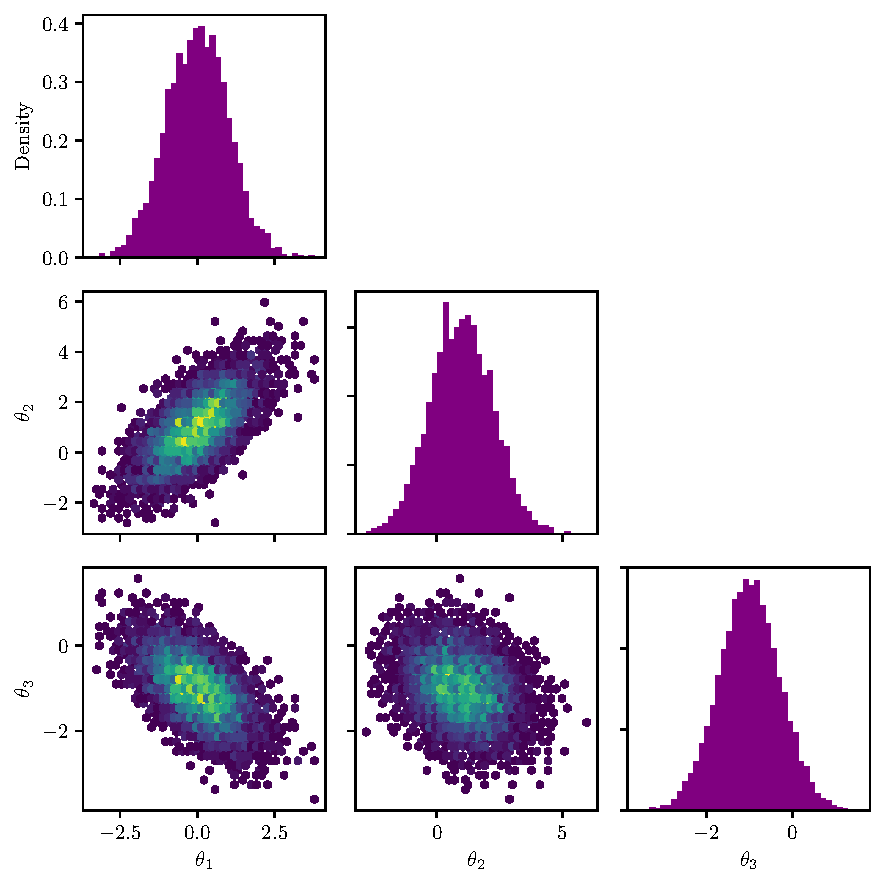
\includegraphics[width=.35\textwidth]{figs/monte-carlo/figure_corner_plot.pdf}
    \caption{A corner plot showing marginal and joint distributions from a Bayesian analysis. Each marginal distribution requires integrating over all other parameters, which is a high-dimensional integration problem.}
    \label{fig:corner-plot}
\end{figure}

By now, the point should be clear that we need to compute high-dimensional integrals to do useful science, but traditional numerical methods fail miserably as dimension increases. This is where Monte Carlo integration offers a way forward. As we will see, unlike grid-based methods, Monte Carlo approaches do not suffer from exponential scaling with dimension. Their convergence rate depends only on the number of samples drawn, not on the dimension of the space, which allows them to be used in high-dimensional problems.

\section{Monte Carlo Integration}

To see the path forward, we must realize that any integral can be written as the size of the integration domain multiplied by the average value of the function over that domain. In particular, consider an integral over some domain $\Omega$ in $N$-dimensional space:
\begin{equation}
    I = \int_{\Omega} f(\mathbf{x}) \, d\mathbf{x}, \quad \mathbf{x} \in \mathbb{R}^N
\end{equation}
We can always rewrite this as
\begin{equation}
    I = \left(\int_{\Omega} 1 \, d\mathbf{x}\right) \langle f \rangle
\end{equation}
where $\langle f \rangle$ is the average value of $f$ over the domain. The first term is just the volume of $\Omega$. The second term is what we need to estimate. To make this precise, we introduce a probability distribution $p(\mathbf{x})$ that is uniform over $\Omega$. This means $p(\mathbf{x}) = 1/V$ for $\mathbf{x} \in \Omega$ and $p(\mathbf{x}) = 0$ otherwise, where $V = \int_{\Omega} 1 \, d\mathbf{x}$ is the volume of the domain. We can then write the average value as an expectation:
\begin{equation}
    \langle f \rangle = \mathbb{E}[f(\mathbf{x})] = \int_{\Omega} f(\mathbf{x}) p(\mathbf{x}) \, d\mathbf{x}
\end{equation}
Since $p(\mathbf{x}) = 1/V$ is constant over $\Omega$, this gives
\begin{equation}
    \langle f \rangle = \frac{1}{V} \int_{\Omega} f(\mathbf{x}) \, d\mathbf{x}
\end{equation}
and therefore $I = V \langle f \rangle$. The Monte Carlo method estimates this expectation using random sampling. We generate a sequence of $M$ points $\mathbf{x}_1, \mathbf{x}_2, \ldots, \mathbf{x}_M$ that are uniformly distributed within $\Omega$. By the law of large numbers, the sample average converges to the true mean as the number of samples increases:
\begin{equation}
    \langle f \rangle = \lim_{M \to \infty} \frac{1}{M} \sum_{i=1}^{M} f(\mathbf{x}_i)
\end{equation}
For a finite number of samples, we estimate the average as
\begin{equation}
    \langle f \rangle_M = \frac{1}{M} \sum_{i=1}^{M} f(\mathbf{x}_i)
\end{equation}
and our Monte Carlo estimate of the integral is
\begin{equation}
    I_{\text{MC}} = V \langle f \rangle_M = \frac{V}{M} \sum_{i=1}^{M} f(\mathbf{x}_i)
\end{equation}

The power of this approach lies in its error scaling. For independent and identically distributed samples, the variance of the sample mean is $\sigma^2/M$, where $\sigma^2$ is the variance of the individual samples. The central limit theorem additionally tells us that this estimator is asymptotically normal. Practically, this means that if you take $M$ random samples, the typical size of the error in $I_{\text{MC}}$ shrinks like $M^{-1/2}$:
\begin{equation}
    I_{\text{MC}} - I \sim M^{-1/2}
\end{equation}

\begin{exampleBox}
    \textbf{Convergence Rate Comparison:} Let's compare the computational effort required to improve a calculation's accuracy by a factor of 10 using different methods. Like we discussed before, for standard grid-based integration like the trapezoidal rule, the error typically scales with the grid spacing $\Delta x$ as $\sim (\Delta x)^2$. To reduce the error by 10, one must decrease $\Delta x$ by $\sqrt{10} \approx 3.16$. In $N$ dimensions, this requires $10^{N/2}$ times more function evaluations. In contrast, the error in the Monte Carlo method scales with the number of samples $M$ as $\sim M^{-1/2}$. To reduce its error by a factor of 10, one simply needs to increase the samples by $10^2 = 100$ times, \emph{regardless of the problem's dimension}.
    
    This dimensional independence is Monte Carlo's main advantage. For a 10-dimensional problem, a grid-based method would need $10^{10/2} = 10^5$ (or 100,000) times more evaluations to achieve the 10x accuracy boost. Monte Carlo, however, would still only need 100 times more samples. If the problem had 20 dimensions, the grid-based method's cost would explode to $10^{10}$ (ten billion) times more evaluations, while Monte Carlo's cost remains fixed at 100 times more samples.
\end{exampleBox}

This dimension-independent convergence rate tames the curse of dimensionality. In low dimensions, carefully designed grid methods can improve faster with each added function evaluation. But as dimension grows, grid methods require exponentially many evaluations to keep shrinking the grid spacing, while Monte Carlo's $M^{-1/2}$ improvement stays the same no matter the dimension. That is why high-dimensional integrals that are intractable with grids become feasible (though still sometimes costly) with Monte Carlo.

Let's work through a classic example that demonstrates the method. We'll compute the area of a circle with diameter 2 (radius 1). This is a problem where we know the exact answer ($\pi$), so we can check our result. The domain $\Omega$ is the square $-1 \leq x_1, x_2 \leq 1$, which has area $V = 4$. We want to integrate the indicator function
\begin{equation}
    f(\mathbf{x}) = H(1 - (x_1^2 + x_2^2))
\end{equation}
where $H$ is the Heaviside step function: $H(z) = 1$ if $z > 0$ and $H(z) = 0$ otherwise. This function equals 1 inside the circle and 0 outside. The integral is
\begin{equation}
    I = \int_{\Omega} f(\mathbf{x}) \, d\mathbf{x} = \text{(area of circle)} = \pi
\end{equation} 
To estimate this with Monte Carlo, we generate $M$ random points uniformly distributed in the square and compute the fraction that fall inside the circle:
\begin{equation}
    \langle f \rangle_M = \frac{1}{M} \sum_{i=1}^{M} f(\mathbf{x}_i) = \frac{\text{number of points inside circle}}{M}
\end{equation}
Our estimate is then
\begin{equation}
    I_{\text{MC}} = V \langle f \rangle_M = 4 \times \frac{\text{number of points inside circle}}{M}
\end{equation}
Here's a simple implementation in MATLAB:
\begin{verbatim}
M = 100;
x = 2 * rand(M, 2) - 1;             % uniform in [-1,1]^2
f = (x(:, 1).^2 + x(:, 2).^2) < 1;  % inside circle? (logical)
fs = mean(f);                       % sample average
I = 4 * fs;                         % scale by domain size, and we have our estimate
\end{verbatim}
Running this code (and visualizing the results), we get something like in Figure~\ref{fig:mc-circle}. With $M=100$ samples, the expected relative error is around 5\%. With $M=10{,}000$ samples, the error drops to around 0.5\% (a factor of 10 improvement in accuracy from 100 times more samples, as predicted by the $M^{-1/2}$ scaling). The convergence of the estimate to the true value (by changing $M$ in the code above) is shown in Figure~\ref{fig:mc-convergence}.
\begin{figure}[htbp]
    \centering
    \begin{subfigure}{0.45\textwidth}
     \centering
     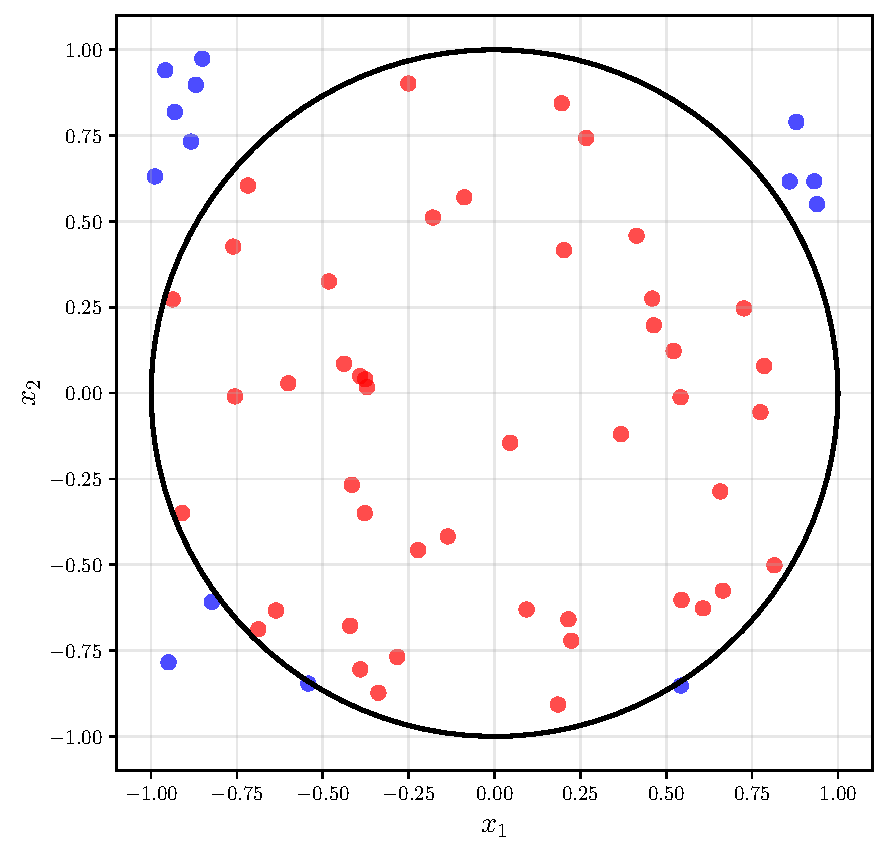
\includegraphics[width=\textwidth]{./figs/monte-carlo/mc_circle.pdf}
     \caption{Monte Carlo estimation of the area of a circle. Random points are uniformly sampled in the enclosing square. Points inside the circle (red) contribute 1 to the integral, points outside (blue) contribute 0.}
     \label{fig:mc-circle}
    \end{subfigure}
    \hfill
    \begin{subfigure}{0.45\textwidth}
     \centering
     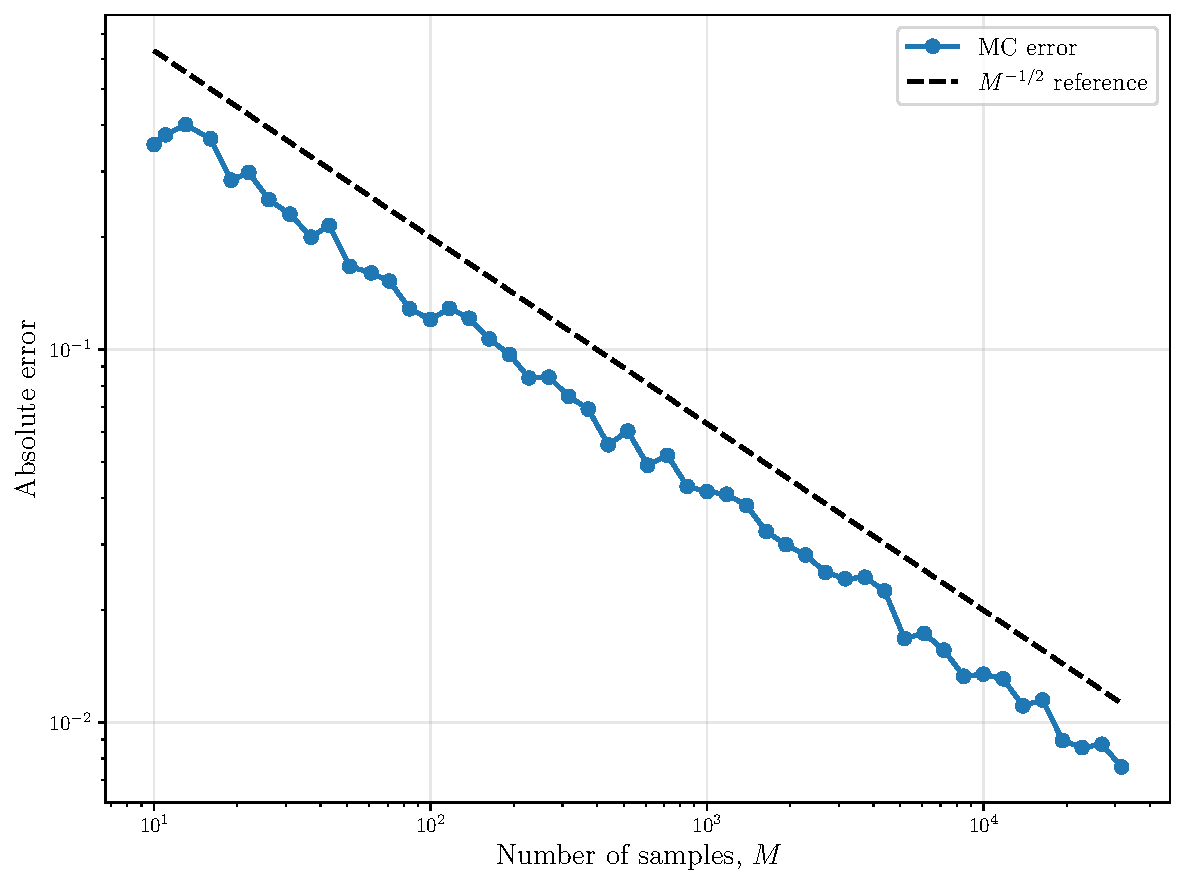
\includegraphics[width=\textwidth]{./figs/monte-carlo/mc_convergence.pdf}
     \caption{Convergence of Monte Carlo integration for estimating the area of a circle. The error decreases as $M^{-1/2}$, so improving accuracy by a factor of 10 requires 100 times more samples. The dimension-independence of this scaling is what makes Monte Carlo practical for high-dimensional problems.}
     \label{fig:mc-convergence}
    \end{subfigure}
    \caption{Monte Carlo integration methods.}
    \label{fig:monte-carlo}
\end{figure}

While Monte Carlo integration breaks the curse of dimensionality, the uniform-sampling approach we've described has some practical limitations. First, when using uniform sampling over a domain $\Omega$, we need to know the volume $V$ of that domain to compute $I = V \langle f \rangle$. For simple domains like hypercubes this is trivial, but for arbitrary domains it may be difficult, and if the domain is the entire space $\mathbb{R}^N$, uniform sampling makes no sense.\footnote{Note: If we already have a normalized probability density $p(\mathbf{x})$ and want to compute $\mathbb{E}_p[f] = \int f(\mathbf{x}) p(\mathbf{x}) \, d\mathbf{x}$, we can sample directly from $p$ and simply average $f(\mathbf{x}_i)$, and no volume factor is needed. This is common in Bayesian applications where we sample from the posterior.} Second, even when the domain is finite, uniform sampling can be extremely inefficient. If the function $f(\mathbf{x})$ has large values only in a small region of the domain (imagine two sharp peaks separated by a vast expanse where $f \approx 0$, as in Figure~\ref{fig:uniform-sampling-problem}) then most of our random samples will land in regions that contribute almost nothing to the integral. We're wasting computational effort evaluating the function where it doesn't matter. Both of these problems have the same solution. Instead of sampling uniformly, we sample from a different probability distribution that concentrates samples where they matter most. This is the idea behind importance sampling.

\begin{figure}[htbp]
    \centering
    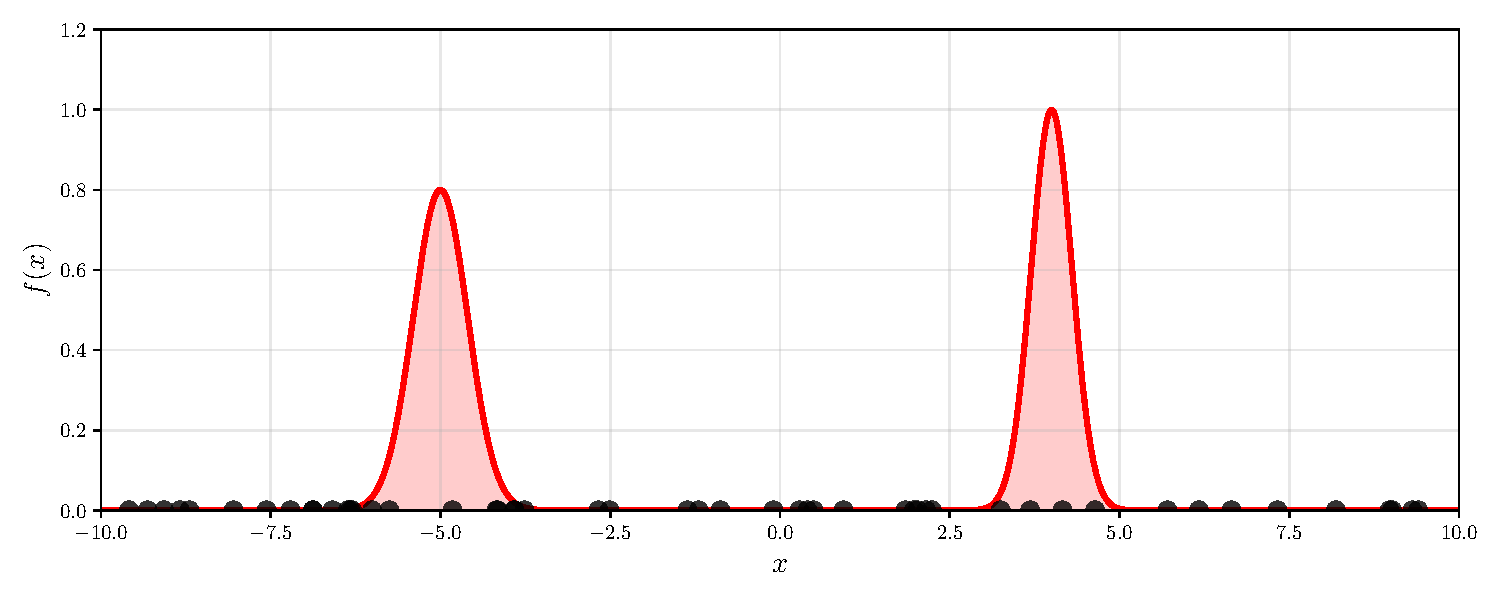
\includegraphics[width=.96\textwidth]{./figs/monte-carlo/uniform_sampling_problem.pdf}
    \caption{The inefficiency of uniform sampling when the integrand has certain characteristics like sharp peaks. Most samples (black dots on the $x$-axis) land in regions where $f(x) \approx 0$, contributing little to the integral estimate. We would get much better accuracy by sampling preferentially near the peaks.}
    \label{fig:uniform-sampling-problem}
\end{figure}

\section{Importance Sampling}
Basic Monte Carlo with uniform sampling works, but it's inefficient when the integrand has structure that we can exploit. Like we mentioned, if $f(\mathbf{x})$ has large values only in small regions of the domain, most uniform samples land where the function is nearly zero and contribute little to the integral, so we should try to sample more near the peaks. Fortunately, we can write any integral as an expectation over more general probability distributions than just the uniform distribution. To see this, we start with the same integral from before, namely
\begin{equation}
    I = \int_{\Omega} f(\mathbf{x}) \, d\mathbf{x}
\end{equation}
and multiply and divide by any probability distribution $p(\mathbf{x})$ that is nonzero wherever $f(\mathbf{x})$ is nonzero:
\begin{equation}
    I = \int_{\Omega} \frac{f(\mathbf{x})}{p(\mathbf{x})} p(\mathbf{x}) \, d\mathbf{x} = \mathbb{E}_{\mathbf{x} \sim p(\mathbf{x})} \left[ \frac{f(\mathbf{x})}{p(\mathbf{x})} \right]
\end{equation}
This is an expectation of the weighted function $f(\mathbf{x})/p(\mathbf{x})$ with respect to the distribution $p(\mathbf{x})$. We can estimate this expectation using Monte Carlo. Generate $M$ samples $\mathbf{x}_1, \mathbf{x}_2, \ldots, \mathbf{x}_M$ from the distribution $p(\mathbf{x})$ (not uniformly!), and compute
\begin{equation}
    I \approx \frac{1}{M} \sum_{i=1}^{M} \frac{f(\mathbf{x}_i)}{p(\mathbf{x}_i)}
\end{equation}
This is importance sampling. Each sample is weighted by $1/p(\mathbf{x}_i)$ to correct for the fact that we're sampling from $p$ rather than uniformly.

\begin{warningBox}
    \textbf{Warning:} It is important to remember that expectation values of functions of random variables depend on the distribution of those random variables. When we write $\mathbb{E}[g(\mathbf{x})]$, we must always be clear about what distribution $\mathbf{x}$ is drawn from. The importance sampling formula works precisely because we're computing the expectation of $f(\mathbf{x})/p(\mathbf{x})$ with $\mathbf{x}$ drawn from $p(\mathbf{x})$.
\end{warningBox}

The obvious question is which distribution $p(\mathbf{x})$ we should choose. We want to minimize the variance of our estimator so that our integral estimate is as reliable as possible. To minimize the estimator's variance, it is enough to minimize the per-sample variance $\text{Var}\left[f(\mathbf{x})/p(\mathbf{x})\right]$, because the variance of our Monte Carlo estimator scales as
\begin{equation}
    \text{Var}\left[\frac{1}{M}\sum_{i=1}^M \frac{f(\mathbf{x}_i)}{p(\mathbf{x}_i)}\right] = \frac{1}{M}\text{Var}\left[\frac{f(\mathbf{x})}{p(\mathbf{x})}\right]
\end{equation}
The per-sample variance is
\begin{equation}
    \text{Var}\left[\frac{f(\mathbf{x})}{p(\mathbf{x})}\right] = \mathbb{E}\left[\left(\frac{f(\mathbf{x})}{p(\mathbf{x})}\right)^2\right] - \left(\mathbb{E}\left[\frac{f(\mathbf{x})}{p(\mathbf{x})}\right]\right)^2 = \mathbb{E}\left[\left(\frac{f(\mathbf{x})}{p(\mathbf{x})}\right)^2\right] - I^2
\end{equation}
where both expectations are with respect to $p(\mathbf{x})$. Expanding the first term,
\begin{equation}
    \mathbb{E}\left[\left(\frac{f(\mathbf{x})}{p(\mathbf{x})}\right)^2\right] = \int_{\Omega} \left(\frac{f(\mathbf{x})}{p(\mathbf{x})}\right)^2 p(\mathbf{x}) \, d\mathbf{x} = \int_{\Omega} \frac{f(\mathbf{x})^2}{p(\mathbf{x})} \, d\mathbf{x}
\end{equation}
To minimize the variance, we need to minimize this integral subject to the constraint that $p(\mathbf{x})$ is a normalized probability distribution. By the Cauchy-Schwarz inequality, we have
\begin{equation}
    \left(\int_{\Omega} \frac{|f(\mathbf{x})|}{p(\mathbf{x})} p(\mathbf{x}) \, d\mathbf{x}\right)^2 \leq \int_{\Omega} \frac{f(\mathbf{x})^2}{p(\mathbf{x})} \, d\mathbf{x} \int_{\Omega} p(\mathbf{x}) \, d\mathbf{x}
\end{equation}
The right-hand side simplifies to $\int f^2/p \, d\mathbf{x}$ since $p$ is normalized. The left-hand side is $\left(\int |f(\mathbf{x})| \, d\mathbf{x}\right)^2$. Equality holds when $|f(\mathbf{x})|$ is proportional to $p(\mathbf{x})$. Therefore, the variance is minimized when
\begin{equation}
p^*(\mathbf{x}) = \frac{|f(\mathbf{x})|}{\int_{\Omega} |f(\mathbf{x})| \, d\mathbf{x}}
\end{equation}
This is the optimal importance sampling distribution. If we sample from $p^*(\mathbf{x})$, the ratio $f(\mathbf{x})/p^*(\mathbf{x})$ is constant up to sign. Specifically, $f(\mathbf{x})/p^*(\mathbf{x}) = \left(\int_\Omega |f(\mathbf{x})| \, d\mathbf{x}\right) \cdot \text{sign}(f(\mathbf{x}))$, which means all samples contribute equally in magnitude to the integral estimate. In the ideal case where $f(\mathbf{x}) \geq 0$ everywhere, we have $p^*(\mathbf{x}) = f(\mathbf{x})/I$ and the variance is exactly zero, which means that every sample gives the same value $I$ when weighted appropriately.\footnote{Note that when $f(\mathbf{x})$ changes sign, the optimal distribution involves $|f(\mathbf{x})|$, but large cancellations between positive and negative contributions can still make the variance large. This is known as the sign problem and is particularly severe in quantum Monte Carlo and other applications (not anything you need to worry about in 10.34).} In practice, the effectiveness of importance sampling is governed entirely by variance control. If $p(\mathbf{x})$ underweights regions where $|f(\mathbf{x})|$ is large, the weights $f/p$ explode and the estimator's variance becomes impractically large.

\begin{exampleBox}
    \textbf{The Catch-22 of Optimal Importance Sampling:} The optimal distribution gives us perfect estimates, but we can't use it without already knowing the answer. When $f(\mathbf{x}) \geq 0$ and we sample from $p^*(\mathbf{x}) = f(\mathbf{x})/I$, every sample gives
    \begin{equation}
    \frac{f(\mathbf{x}_i)}{p^*(\mathbf{x}_i)} = \frac{f(\mathbf{x}_i)}{f(\mathbf{x}_i)/I} = I
    \end{equation}
    The estimate is exactly $I$ with \emph{zero variance}. But to construct $p^*$, we need its normalization constant, which is precisely $I$, the integral we're trying to compute!
    
    For a concrete example, suppose we want to compute $I = \int_0^1 e^x \, dx$. The optimal importance sampling distribution is
    \begin{equation}
    p^*(x) = \frac{e^x}{\int_0^1 e^x \, dx} = \frac{e^x}{e - 1}
    \end{equation}
    Notice how we had to compute the normalization constant to construct $p^*$, and the normalization constant required knowing the very integral we're trying to compute. If we already knew $I = e - 1$, we wouldn't need to run Monte Carlo integration in the first place. This paradox means that in practice, we seek distributions that approximate $|f(\mathbf{x})|$ without requiring knowledge of $I$. For instance, we might use $p(\mathbf{x}) \propto |f(\mathbf{x})|$ with a tractable normalization or concentrate samples where we expect $|f(\mathbf{x})|$ to be large.
\end{exampleBox}
So we can't actually use the optimal importance sampling distribution in practice, but all is not lost, as we can uncover some useful information by looking at its form. Indeed, the optimal distribution shows us that our strategy should be to choose $p(\mathbf{x})$ to be roughly proportional to $|f(\mathbf{x})|$. And as we saw in the example above, we must choose a distribution that approximates this without requiring knowledge of the integral we're computing (or else there would be no need for MC sampling in the first place). For example, if $f(\mathbf{x})$ has sharp peaks at known locations, we might choose a Gaussian mixture centered on those peaks. If $f(\mathbf{x}) = \exp(-U(\mathbf{x}))$ for some energy function $U$, we might sample from a simpler distribution with similar structure.

Here's the importance sampling algorithm:

\begin{algorithmBox}
    \textbf{Importance sampling for computing} $I = \int_{\Omega} f(\mathbf{x}) \, d\mathbf{x}$:
    \begin{enumerate}
        \item Choose an importance distribution $p(\mathbf{x})$ that is nonzero wherever $f(\mathbf{x}) \neq 0$ (try to match the structure of $f(\mathbf{x})$ as closely as possible)
        \item Generate $M$ samples $\mathbf{x}_1, \mathbf{x}_2, \ldots, \mathbf{x}_M$ from $p(\mathbf{x})$
        \item Compute the weighted average:
        \begin{equation}
            I \approx \frac{1}{M} \sum_{i=1}^{M} \frac{f(\mathbf{x}_i)}{p(\mathbf{x}_i)}
        \end{equation}
    \end{enumerate}
\end{algorithmBox}

% MC: should put a concrete example of importance sampling here (Gaussian mixture for two peaks would flow well here)

This gives us a numerical recipe for approximating integrals more efficiently than uniform sampling. But there's a practical problem here: how do we actually generate samples from $p(\mathbf{x})$? For a uniform distribution, this is trivial; we can use any programming language's uniform random number generator. But for an arbitrary probability distribution, especially in multiple dimensions, sampling is nontrivial.

\paragraph*{Sampling from Arbitrary Discrete Distributions}
In the discrete case, we can sample from any target distribution using only a uniform random number generator. Let's see how this works with a concrete example. Imagine we have 5 possible outcomes (labeled 0 through 4) with the following probabilities:
\begin{center}
\begin{tabular}{c|ccccc}
Outcome & 0 & 1 & 2 & 3 & 4 \\
\hline
Probability & 0.10 & 0.15 & 0.25 & 0.30 & 0.20
\end{tabular}
\end{center}
The method, called the discrete inverse transform method, works in two main stages. First, we pre-compute the cumulative distribution by summing the probabilities. This creates a series of ``bins'' that divide the interval $[0, 1]$:
\begin{center}
\begin{tabular}{c|ccccc}
Outcome & 0 & 1 & 2 & 3 & 4 \\
\hline
Cumulative & 0.10 & 0.25 & 0.50 & 0.80 & 1.00
\end{tabular}
\end{center}
Each outcome now corresponds to a sub-interval: outcome 0 gets $[0, 0.10)$, outcome 1 gets $[0.10, 0.25)$, outcome 2 gets $[0.25, 0.50)$, and so on. Notice that the size of each bin is exactly equal to its target probability.
\begin{center}
    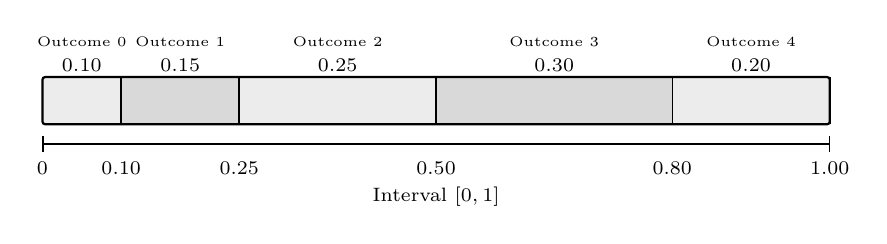
\begin{tikzpicture}[x=10cm,y=1cm]
        %--- styling ---
        \def\H{0.6} % bar height
      
        %--- filled bins (widths match probabilities) ---
        \fill[gray!15]   (0,0)      rectangle (0.10,\H); % outcome 0 (0.10)
        \fill[gray!30]   (0.10,0)   rectangle (0.25,\H); % outcome 1 (0.15)
        \fill[gray!15]   (0.25,0)   rectangle (0.50,\H); % outcome 2 (0.25)
        \fill[gray!30]   (0.50,0)   rectangle (0.80,\H); % outcome 3 (0.30)
        \fill[gray!15]   (0.80,0)   rectangle (1.00,\H); % outcome 4 (0.20)
      
        %--- outer frame of [0,1] interval ---
        \draw[line width=0.8pt, rounded corners=1pt] (0,0) rectangle (1,\H);
      
        %--- cumulative cut lines and tick labels ---
        \foreach \x/\lab in {0/0, 0.10/0.10, 0.25/0.25, 0.50/0.50, 0.80/0.80, 1.00/1.00} {
          \draw[line width=0.6pt] (\x,0) -- (\x,\H);
          \node[below=10pt] at (\x,0) {\scriptsize \lab};
        }
      
        %--- outcome + probability labels (centered in bins) ---
        \node at (0.05,  \H+0.45) {\tiny Outcome 0};
        \node at (0.05,  \H+0.15) {\scriptsize $0.10$};
      
        \node at (0.175, \H+0.45) {\tiny Outcome 1};
        \node at (0.175, \H+0.15) {\scriptsize $0.15$};
      
        \node at (0.375, \H+0.45) {\tiny Outcome 2};
        \node at (0.375, \H+0.15) {\scriptsize $0.25$};
      
        \node at (0.65,  \H+0.45) {\tiny Outcome 3};
        \node at (0.65,  \H+0.15) {\scriptsize $0.30$};
      
        \node at (0.90,  \H+0.45) {\tiny Outcome 4};
        \node at (0.90,  \H+0.15) {\scriptsize $0.20$};
      
        %--- axis annotation ---
        \draw[|-|] (0,-0.250) -- (1,-0.250) node[midway, below=12pt] {\scriptsize Interval $[0,1]$};
      \end{tikzpicture}
\end{center}
Second, to generate a sample, we draw a single random number $u$ uniformly from $[0,1]$ (i.e., $u \sim \mathcal{U}(0,1)$) and find which bin $u$ falls into. For example, if we draw $u = 0.65$, we look at our cumulative table. Since $0.65$ is greater than $0.50$ (the top of bin 2) but less than or equal to $0.80$ (the top of bin 3), our sample falls into bin 3. We return outcome 3. This works because the probability of $u$ landing in any specific bin is equal to the bin's width, which we designed to be the outcome's target probability. For instance, the probability of $u$ falling in the range $[0.50, 0.80)$ is $0.80 - 0.50 = 0.30$, which is exactly the probability we wanted for outcome 3. 

Figure~\ref{fig:discrete-sampling-mc} illustrates this process. The left panel shows the target probabilities, and the right panel shows the cumulative distribution (the bins that we compute by summing the probabilities). Our random draw $u = 0.65$ lands in the interval corresponding to outcome 3. If we keep repeating this process, we will generate outcomes with the correct frequencies according to our target distribution. To be explicit here, calling our discrete target distribution's PMF $p(x)$ and its CDF $F(x)$, we are saying that this procedure maps a uniform random number $u$ to a sample $x \sim p(x)$ via the relation $x = F^{-1}(u)$.

\begin{figure}[htbp]
    \centering
    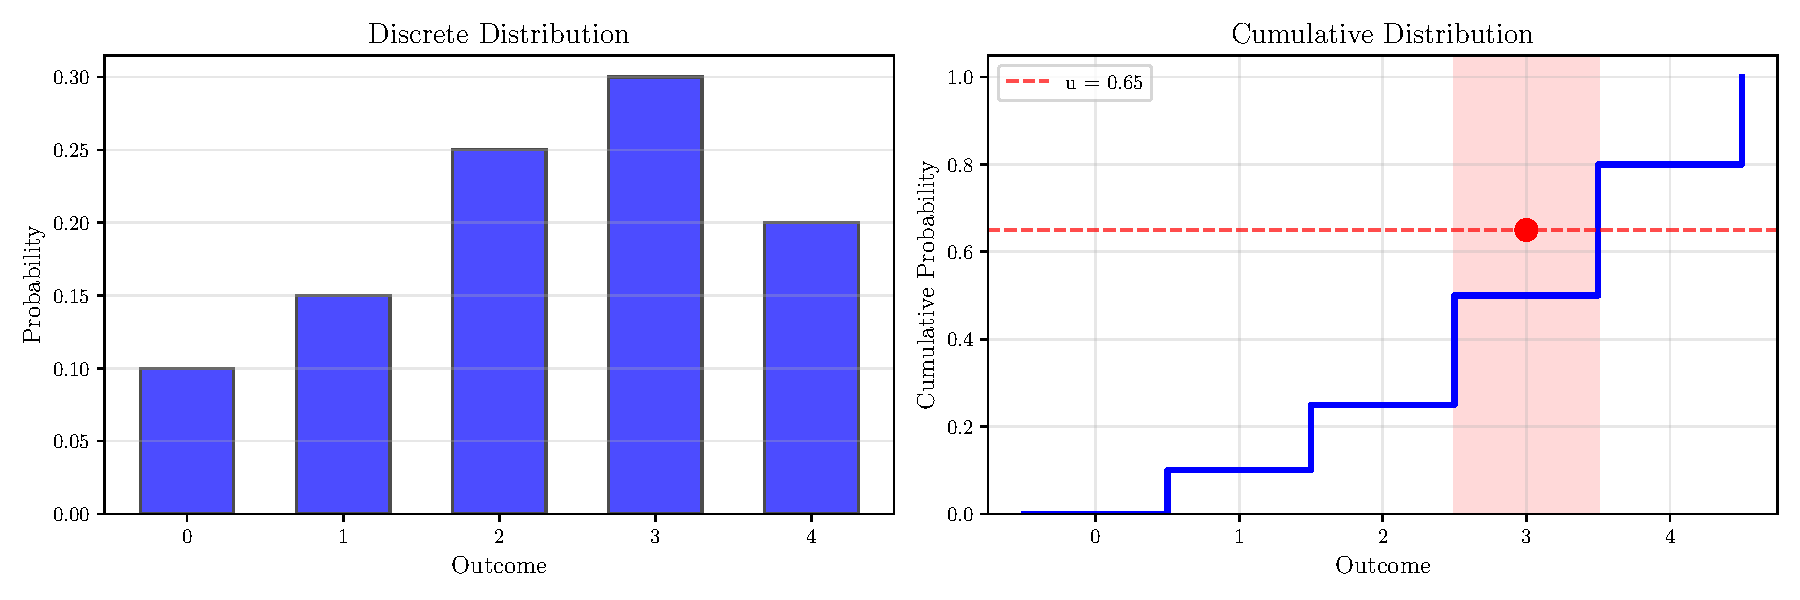
\includegraphics[width=0.98\textwidth]{./figs/monte-carlo/discrete_sampling.pdf}
    \caption{Sampling from a discrete distribution. We draw $u \sim \mathcal{U}(0,1)$ and find the bin where the cumulative distribution exceeds $u$. Here, $u=0.65$ falls into the bin for outcome 3.}
    \label{fig:discrete-sampling-mc}
\end{figure}

\paragraph*{Sampling from Arbitrary Continuous Distributions}
The same idea extends to continuous distributions. Suppose we want to sample from a continuous PDF $p(x)$. The sampling process is analogous to the discrete case:
\begin{enumerate}
    \item Draw a random number $u$ uniformly from $[0,1]$ (i.e., $u \sim \mathcal{U}(0,1)$).
    \item Compute the corresponding $x$ by inverting the CDF: $x = F^{-1}(u)$.
\end{enumerate}
This value $x$ is our sample drawn from the distribution $p(x)$.

Why does this work? The CDF $F(x)$ maps $x$-values to probabilities in $[0,1]$. Since it's monotonically increasing, its inverse $F^{-1}(u)$ exists and maps uniform probabilities from $[0,1]$ back to $x$-values. We can show this formally by checking the cumulative probability of our generated sample $x$:
\begin{equation}
    P(x \leq a) = P(F^{-1}(u) \leq a)
\end{equation}
Applying $F$ to both sides of the inequality (which preserves the relation since $F$ is increasing), we get
\begin{equation}
    P(u \leq F(a)) = F(a)
\end{equation}
The final equality holds because $u$ is uniform on $[0,1]$, so the probability of $u$ being less than some value $v$ is simply $v$. Since the resulting sample $x$ has the cumulative distribution $F(a)$, it must be distributed according to the original density $p(x)$.\footnote{This argument assumes $F$ is strictly increasing so that $F^{-1}$ is well-defined. For distributions with flat regions or discrete jumps, we define $F^{-1}(u)$ as the smallest $x$ with $F(x) \geq u$, which still works.}

Figure~\ref{fig:inverse-transform} shows this for a bimodal distribution. The right panel shows the CDF $F(x)$. We draw $u = 0.7$ on the $y$-axis, find its corresponding point on the curve, and map it down to the $x$-axis to get our sample $x$. This process correctly maps uniform draws into regions of high probability density.

\begin{figure}[htbp]
    \centering
    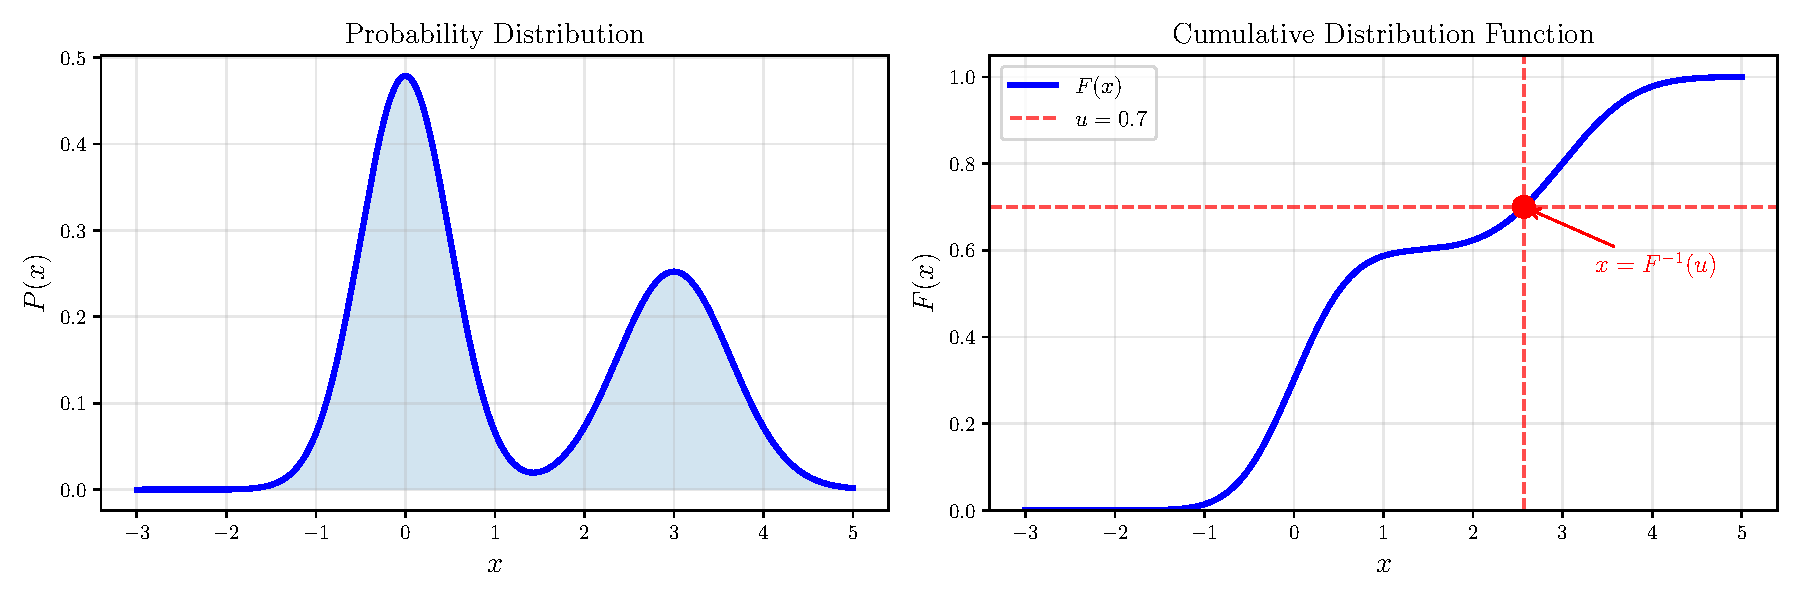
\includegraphics[width=0.98\textwidth]{./figs/monte-carlo/inverse_transform.pdf}
    \caption{Inverse transform sampling in one dimension. The CDF $F(x)$ maps the domain of $x$ to $[0,1]$. Its inverse $F^{-1}(u)$ maps uniform random numbers $u$ back to samples $x$ from the target distribution $p(x)$.}
    \label{fig:inverse-transform}
\end{figure}

Despite its simplicity, the inverse transform method has major practical limitations:
\begin{itemize}
    \item The inverse CDF $F^{-1}$ is often hard to compute. For many common distributions (like the Gaussian or the bimodal example in the figure), $F(x)$ and its inverse $F^{-1}(u)$ cannot be written in a simple closed form. In these cases, we must use expensive numerical root-finding to solve $F(x) = u$ or use a pre-computed lookup table, which requires storage and interpolation.
    \item The method does not extend well to high dimensions. For multivariate distributions in $\mathbb{R}^N$, there is no unique or simple way to define a CDF and its inverse. While we could use this method for $N$ independent variables, most interesting problems involve complex dependencies.
\end{itemize}
Still, inverse transform sampling is extremely fast for discrete distributions (requiring just a binary search on the cumulative table) and is the method of choice for any 1D continuous distribution (like the exponential distribution) where $F^{-1}$ has an efficient closed-form expression. For high-dimensional problems, more sophisticated techniques are available.

\section{\texorpdfstring{Rejection Sampling\textsuperscript{*}}{Rejection Sampling}}
While inverse transform sampling is elegant and exact, we saw that it has the major limitation that we need to analytically compute and invert the cumulative distribution function. For many distributions, especially with complex functional forms, this is practically impossible. Rejection sampling gives us a complementary approach that works for any distribution we can evaluate, even if we cannot integrate it. Importantly, rejection sampling does not require the target distribution $p(\mathbf{x})$ to be normalized. We only need to be able to evaluate something proportional to $p(\mathbf{x})$, which is often much easier to do. Rejection sampling is best understood from a geometric perspective. Instead of transforming uniform samples through the CDF, we uniformly sample from a region that encloses the target distribution and then randomly ``reject'' points to sculpt out the desired shape (see \autoref{fig:rejection-overview} for a 1D example).

\begin{figure}[htbp]
    \centering
    % helper: the "target pdf" squiggle, reused in all three panels
    \newcommand{\targetcurve}{%
        % fill without bottom line
        \fill[blue!70!cyan,opacity=0.3]
            (0,0)
            .. controls (0.5,0.3) and (1,1.0) .. (1.2,1.5)
            .. controls (1.5,2.5) and (2.0,2.7) .. (2.5,2.9)
            .. controls (3.0,3.4) and (3.5,3.0) .. (4.0,2.2)
            .. controls (4.5,2.0) and (5.0,2.3) .. (5.4,2.5)
            .. controls (5.8,2.7) and (6.2,2.6) .. (6.5,2.2)
            .. controls (6.8,1.4) and (7.0,1.0) .. (7.2,0.8)
            .. controls (7.6,0.4) and (8.0,0.3) .. (8.4,0.5)
            .. controls (8.8,0.7) and (9.0,1.0) .. (9.2,1.2)
            .. controls (9.6,1.6) and (9.8,1.8) .. (10,1.7)
            -- (10,0) -- cycle;
        % draw only the top curve
        \draw[very thick,blue!70!cyan]
            (0,0)
            .. controls (0.5,0.3) and (1,1.0) .. (1.2,1.5)
            .. controls (1.5,2.5) and (2.0,2.7) .. (2.5,2.9)
            .. controls (3.0,3.4) and (3.5,3.0) .. (4.0,2.2)
            .. controls (4.5,2.0) and (5.0,2.3) .. (5.4,2.5)
            .. controls (5.8,2.7) and (6.2,2.6) .. (6.5,2.2)
            .. controls (6.8,1.4) and (7.0,1.0) .. (7.2,0.8)
            .. controls (7.6,0.4) and (8.0,0.3) .. (8.4,0.5)
            .. controls (8.8,0.7) and (9.0,1.0) .. (9.2,1.2)
            .. controls (9.6,1.6) and (9.8,1.8) .. (10,1.7);
    }

    % same curve but not closed/filled, just outline (for middle/right panels)
    \newcommand{\targetoutline}{%
        \draw[very thick,blue!70!cyan]
            (0,0)
            .. controls (0.5,0.3) and (1,1.0) .. (1.2,1.5)
            .. controls (1.5,2.5) and (2.0,2.7) .. (2.5,2.9)
            .. controls (3.0,3.4) and (3.5,3.0) .. (4.0,2.2)
            .. controls (4.5,2.0) and (5.0,2.3) .. (5.4,2.5)
            .. controls (5.8,2.7) and (6.2,2.6) .. (6.5,2.2)
            .. controls (6.8,1.4) and (7.0,1.0) .. (7.2,0.8)
            .. controls (7.6,0.4) and (8.0,0.3) .. (8.4,0.5)
            .. controls (8.8,0.7) and (9.0,1.0) .. (9.2,1.2)
            .. controls (9.6,1.6) and (9.8,1.8) .. (10,1.7)
            -- (10,0);
    }

    \begin{subfigure}[t]{0.31\textwidth}
        \centering
        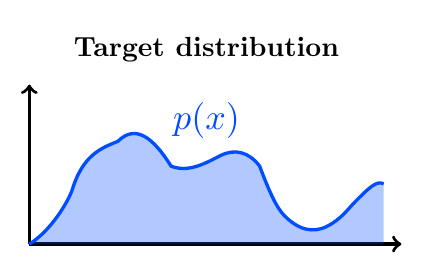
\begin{tikzpicture}[scale=0.45]
            \draw[very thick,->] (0,0) -- (0,4.5);
            \draw[very thick,->] (0,0) -- (10.5,0);
            \targetcurve
            \node[blue!70!cyan,scale=1.3] at (5,3.5) {$p(x)$};
            \node[align=center,scale=1.0,font=\bfseries] at (5,5.5) {Target distribution};
        \end{tikzpicture}
    \end{subfigure}\hfill%
    \begin{subfigure}[t]{0.31\textwidth}
        \centering
        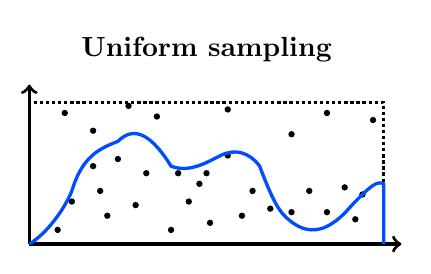
\begin{tikzpicture}[scale=0.45]
            \draw[very thick,->] (0,0) -- (0,4.5);
            \draw[very thick,->] (0,0) -- (10.5,0);
            \draw[densely dotted,very thick] (0,0) rectangle (10,4);
            \foreach \x/\y in {
                0.8/0.4, 1.2/1.2, 1.8/2.2, 2.5/2.4, 3.0/1.1,
                4.2/2.0, 4.8/1.7, 5.1/0.6, 5.6/2.5,
                6.3/1.5, 6.8/1.0, 7.4/0.9, 7.9/1.5,
                8.4/0.9, 8.9/1.6, 9.4/1.4, 2.2/0.8,
                3.3/2.0, 4.0/0.4, 6.0/0.8, 5.0/2.0,
                4.5/1.2, 2.0/1.5, 9.2/0.7,
                1.0/3.7, 2.8/3.9, 3.6/3.6, 5.6/3.8,
                7.4/3.1, 8.4/3.7, 9.7/3.5, 1.8/3.2}
            {
                \fill (\x,\y) circle (0.09);
            }
            \targetoutline
            \node[align=center,scale=1.0,font=\bfseries] at (5,5.5) {Uniform sampling};
        \end{tikzpicture}
    \end{subfigure}\hfill%
    \begin{subfigure}[t]{0.31\textwidth}
        \centering
        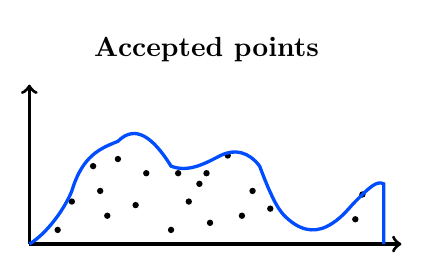
\begin{tikzpicture}[scale=0.45]
            \draw[very thick,->] (0,0) -- (0,4.5);
            \draw[very thick,->] (0,0) -- (10.5,0);
            \foreach \x/\y in {
                0.8/0.4, 1.2/1.2, 1.8/2.2, 2.5/2.4, 3.0/1.1,
                4.2/2.0, 4.8/1.7, 5.1/0.6, 5.6/2.5,
                6.3/1.5, 6.8/1.0, 9.4/1.4, 2.2/0.8,
                3.3/2.0, 4.0/0.4, 6.0/0.8, 5.0/2.0,
                4.5/1.2, 2.0/1.5, 9.2/0.7}
            {
                \fill (\x,\y) circle (0.09);
            }
            \targetoutline
            \node[align=center,scale=1.0,font=\bfseries] at (5,5.5) {Accepted points};
        \end{tikzpicture}
    \end{subfigure}
    
    \caption{The rejection sampling process. We generate many samples uniformly, then accept only those that appropriately represent the target distribution $p(\mathbf{x})$.}
    \label{fig:rejection-overview}
\end{figure}

The method works as follows. We need a proposal distribution $q(\mathbf{x})$ that we can easily sample from (typically uniform) and a constant $M$ such that the target distribution is always bounded by the scaled proposal:
\begin{equation}
    p(\mathbf{x}) \le M q(\mathbf{x}) \quad \forall \mathbf{x} \in \Omega
\end{equation}
This ensures that $M q(\mathbf{x})$ forms an envelope over $p(\mathbf{x})$ (in the 1D example shown in \autoref{fig:rejection-overview}, the bound $M q(\mathbf{x})$ is a the black dotted line (a constant) since we are using a uniform proposal distribution). For each proposed sample $\mathbf{x}_i$ drawn from $q(\mathbf{x})$, we generate a uniform random number $u_i \in [0,1]$ and accept the sample if
\begin{equation}
u_i < \frac{p(\mathbf{x}_i)}{M q(\mathbf{x}_i)}
\end{equation}
Otherwise, we discard it and try again. The accepted samples are distributed according to $p(\mathbf{x})$.

\begin{algorithmBox}
    \textbf{Rejection sampling algorithm:}
    \begin{enumerate}
        \item Choose a proposal distribution $q(\mathbf{x})$ that is easy to sample from (e.g., uniform)
        \item Find a constant $M$ such that $p(\mathbf{x}) \le M q(\mathbf{x})$ for all $\mathbf{x}$ in the domain
        \item Generate a sample $\mathbf{x}_i$ from $q(\mathbf{x})$
        \item Generate a uniform random number $u_i \in [0,1]$
        \item If $u_i < p(\mathbf{x}_i)/(M q(\mathbf{x}_i))$, accept $\mathbf{x}_i$ as a sample from $p(\mathbf{x})$
        \item Otherwise, reject $\mathbf{x}_i$ and return to step 3
        \item Repeat until the desired number of accepted samples is obtained
    \end{enumerate}
\end{algorithmBox}

To see how this works in practice, let's consider a simple example. We want to draw 100 samples from a distribution on $[-1, +1]$ where $p(x < 0) = 1/3$ and $p(x > 0) = 2/3$, with the distribution uniform within each region. We can write this as
\begin{equation}
p(x) = \frac{1}{3} H(-x) + \frac{2}{3} H(x)
\end{equation}
where $H$ is the Heaviside function. We'll use a uniform proposal distribution $q(x) = 1/2$ on $[-1,1]$. To satisfy $p(x) < M q(x)$ everywhere, we need $M = 4/3$, giving $M q(x) = 2/3$. We implement this in Python and show the results in \autoref{fig:rejection-convergence}. With only 100 accepted samples, the histogram shows the general structure but with significant noise. With 10,000 accepted samples, the empirical distribution closely matches the target, with approximately 1/3 of samples in the negative region and 2/3 in the positive region.

\begin{figure}[htbp]
    \centering
    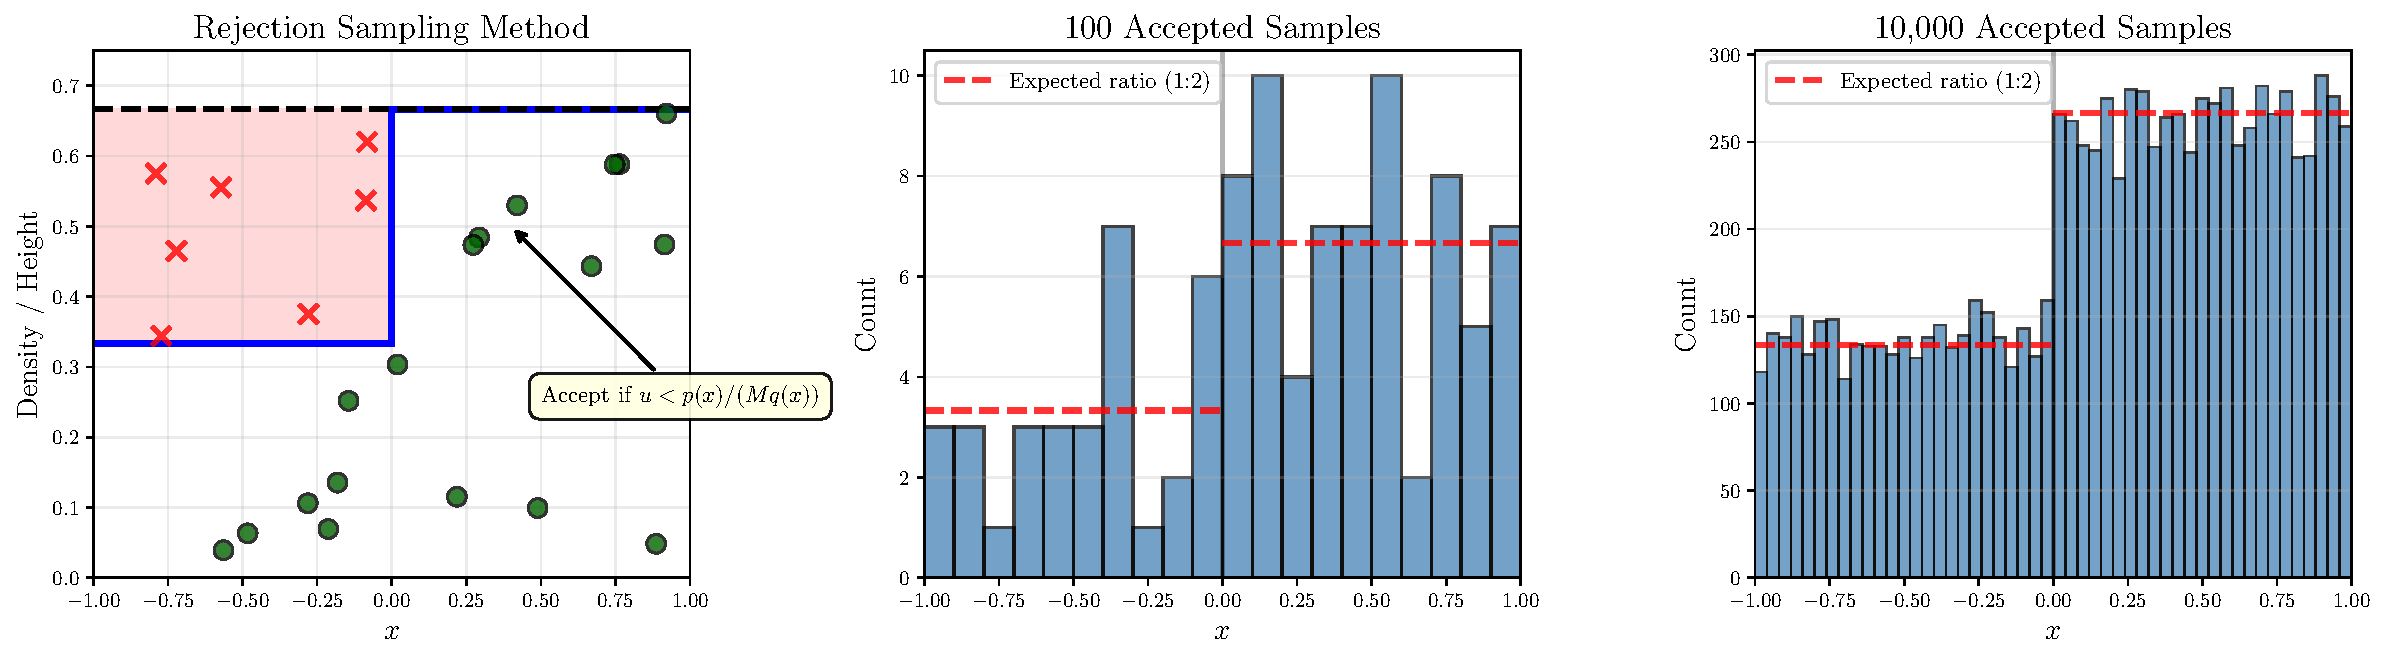
\includegraphics[width=.98\textwidth]{./figs/monte-carlo/rejection_convergence.pdf}
    \caption{Rejection sampling from a piecewise-constant target $p(x)$ using a uniform proposal on $[-1,1]$ and envelope $Mq(x)$. Left: 100 accepted samples give an empirical split of $32/68$ between $x<0$ and $x>0$ (target $1/3$ vs.\ $2/3$). Right: with 10{,}000 accepted samples ($3428/6572$), the histogram aligns closely with the theoretical piecewise densities. The dashed lines show the expected per-bin counts; points above the envelope (rejected proposals) illustrate the accept/reject rule.}
    \label{fig:rejection-convergence}
\end{figure}

While rejection sampling is conceptually simple and works for arbitrary distributions, it has significant practical limitations. The first problem is finding an appropriate bound. We need to choose a proposal distribution $q(\mathbf{x})$ and constant $M$ such that $p(\mathbf{x}) \le M q(\mathbf{x})$ everywhere. For complex distributions, especially in high dimensions, this can be difficult. If $p(\mathbf{x})$ has sharp peaks or heavy tails, we may need a very large $M$ to ensure the inequality holds everywhere. This leads to the second, more serious problem of computational efficiency. The acceptance probability for each proposed sample is $p(\mathbf{x}_i)/(M q(\mathbf{x}_i))$. If $M$ is large, most proposals are rejected. In the worst case, if $p(\mathbf{x})$ is concentrated in a tiny region while $M q(\mathbf{x})$ must cover a vast domain, we might reject 99.99\% of proposals or more. Each rejection wastes a random number generation and a function evaluation. To obtain $N$ accepted samples, we typically need on the order of $N \times M$ proposals, which can be prohibitively expensive.

In high dimensions, both problems become severe. The volume of high-dimensional spaces grows exponentially, making it hard to find tight bounds, and the rejection rate can become astronomical. For the problems we actually care about (sampling from posterior distributions in Bayesian inference, computing partition functions in statistical mechanics, exploring configuration spaces of molecules, etc.), rejection sampling is generally impractical. The solution is Markov Chain Monte Carlo, which we'll develop next. This method avoids the need for a bounding envelope and can efficiently explore high-dimensional distributions by constructing a sequence of samples where each new sample depends only on the previous one.

\section{Markov chain Monte Carlo}

Both the inverse transform method and rejection sampling are generally impractical in high dimensions. Markov chain Monte Carlo (MCMC) fixes this by taking a completely different approach than both of these methods. Instead of generating independent samples, we construct a sequence of correlated samples where each new sample depends only on the previous one. This seemingly simple idea leads to powerful algorithms that can efficiently explore high-dimensional probability distributions.

\subsection{Markov Chains}
A sequence of random variables $\mathbf{x}_1, \mathbf{x}_2, \mathbf{x}_3, \ldots, \mathbf{x}_M$ forms a Markov chain if the probability of each state depends only on the immediately preceding state. In general, the joint probability of a sequence factors as
\begin{equation}
    P(\mathbf{x}_1, \mathbf{x}_2, \mathbf{x}_3, \ldots, \mathbf{x}_M) = P(\mathbf{x}_1) P(\mathbf{x}_2|\mathbf{x}_1) P(\mathbf{x}_3|\mathbf{x}_2, \mathbf{x}_1) \cdots P(\mathbf{x}_M|\mathbf{x}_{M-1}, \ldots, \mathbf{x}_2, \mathbf{x}_1)
\end{equation}
The sequence is a Markov chain if it satisfies the Markov property:
\begin{equation}
    P(\mathbf{x}_i|\mathbf{x}_{i-1}, \ldots, \mathbf{x}_2, \mathbf{x}_1) = P(\mathbf{x}_i|\mathbf{x}_{i-1}), \quad i = 2, 3, \ldots, M
\end{equation}
The conditional probability $P(\mathbf{x}_i|\mathbf{x}_{i-1})$ describes the likelihood of observing a value $\mathbf{x}_i$ at step $i$ given the value $\mathbf{x}_{i-1}$ at step $i-1$. The future depends only on the present, not on the past.

Markov chains appear throughout science. The panels in \autoref{fig:markov-examples} give two such cases. \autoref{fig:markov-examples-a} shows a discrete-state chain used for disease progression: the chain moves between Healthy and Sick with the indicated transition probabilities, and the state Dead is absorbing (once entered, it cannot be left). \autoref{fig:markov-examples-b} shows a continuous-state process (Brownian motion): the next position depends only on the current position. Formally,
\begin{equation}
    p(\mathbf{x}_{t+\Delta t}\,|\,\mathbf{x}_t) \sim \mathcal{N}\!\big(\mathbf{x}_t,\; \alpha\, \Delta t\, \mathbf{I}\big),
\end{equation}
where $\alpha$ is the diffusion coefficient. Both panels highlight the Markov property, which is that the future is conditionally independent of the past given the present.

\begin{figure}[htbp]
    \centering

    %---------------------------------
    % (a) Discrete Markov chain
    %---------------------------------
    \begin{subfigure}[t]{0.47\textwidth}
    \centering
    \begin{tikzpicture}[
        >=Latex,
        state/.style={
            draw,
            rounded corners=4pt,
            minimum width=2.2cm,
            minimum height=1cm,
            font=\small,
            align=center
        },
        arrow/.style={-{Latex[length=3mm]}, thick},
        prob/.style={font=\scriptsize, midway, sloped, above}
    ]

    % Nodes
    \node[state, fill=green!10]                        (healthy) {Healthy};
    \node[state, fill=yellow!10, right=2.8cm of healthy] (sick)    {Sick};
    \node[state, fill=red!10,    below=1.8cm of sick]    (dead)    {Dead\\(absorbing)};

    % Self-loops and transitions (use edges for clean geometry)
    \path[->]
        (healthy) edge[loop above] node[font=\scriptsize, yshift=1mm] {$0.9$} (healthy)
        (sick)    edge[loop above] node[font=\scriptsize, yshift=1mm] {$0.5$} (sick)
        (dead)    edge[loop below] node[font=\scriptsize, yshift=-1mm] {$1.0$} (dead)
        (healthy) edge node[prob] {$0.1$} (sick)
        (sick.south) edge[bend left=15] node[prob] {$0.3$} (healthy.south)
        (sick) edge node[prob] {$0.2$} (dead);

    \end{tikzpicture}

    \caption{Discrete Markov chain (disease progression). Each arrow shows the probability of jumping to the next state in one step. ``Dead'' is absorbing: once there, you never leave.}
    \label{fig:markov-examples-a}
    \end{subfigure}
    \hfill
    %---------------------------------
    % (b) Continuous Markov process
    %---------------------------------
    \begin{subfigure}[t]{0.47\textwidth}
    \centering
    \begin{tikzpicture}[
        dot/.style={circle, fill=black, inner sep=1pt},
        arrow/.style={thick, -{Latex[length=3mm]}},
        axis/.style={thin, gray}
    ]

    % Axes to suggest 2D space
    \draw[axis] (-0.5,0) -- (4.2,0) node[below right, font=\scriptsize] {$x$};
    \draw[axis] (0,-0.5) -- (0,4.2) node[above left,  font=\scriptsize] {$y$};

    % Random walk points (hand-picked)
    \coordinate (p0) at (0.5,0.6);
    \coordinate (p1) at (1.2,1.1);
    \coordinate (p2) at (1.0,2.0);
    \coordinate (p3) at (1.8,2.5);
    \coordinate (p4) at (2.4,2.0);
    \coordinate (p5) at (3.2,2.4);

    % Path arrows
    \draw[arrow] (p0) -- (p1);
    \draw[arrow] (p1) -- (p2);
    \draw[arrow] (p2) -- (p3);
    \draw[arrow] (p3) -- (p4);
    \draw[arrow] (p4) -- (p5);

    % Dots and time labels
    \node[dot, label={[font=\scriptsize]below left:$\mathbf{x}_{t_0}$}] at (p0) {};
    \node[dot, label={[font=\scriptsize]above right:$\mathbf{x}_{t_1}$}] at (p1) {};
    \node[dot, label={[font=\scriptsize]left:$\mathbf{x}_{t_2}$}]       at (p2) {};
    \node[dot, label={[font=\scriptsize]above:$\mathbf{x}_{t_3}$}]      at (p3) {};
    \node[dot, label={[font=\scriptsize]below:$\mathbf{x}_{t_4}$}]      at (p4) {};
    \node[dot, label={[font=\scriptsize]right:$\mathbf{x}_{t_5}$}]      at (p5) {};

    % Local Gaussian "cloud" around p3 to suggest conditional step distribution
    \draw[gray, very thin, dashed] (p3) circle [x radius=0.5cm, y radius=0.3cm, rotate=20];
    \node[font=\scriptsize, gray, align=center] at ($(p3)+(0.9,0.4)$)
        {$p(\mathbf{x}_{t+1}|\mathbf{x}_t)$ \\ $\sim \mathcal{N}(\mathbf{x}_t,\alpha \Delta t \mathbf{I})$};

    \end{tikzpicture}

    \caption{Continuous-state Markov process (Brownian motion / diffusion). Each new position depends only on the immediately previous one.}
    \label{fig:markov-examples-b}
    \end{subfigure}

    \caption{Examples of Markov chains / processes.}
    \label{fig:markov-examples}
\end{figure}

The conditional probability $P(\mathbf{x}_i|\mathbf{x}_{i-1})$ is the transition probability density that governs movement between states $\mathbf{x}_{i-1}$ and $\mathbf{x}_i$. If this transition probability is independent of $i$, the Markov chain is homogeneous. For a homogeneous chain, we write the transition probability as
\begin{equation}
    P(\mathbf{x}_i|\mathbf{x}_{i-1}) = T(\mathbf{x}_i, \mathbf{x}_{i-1})
\end{equation}
where $T(\mathbf{x}, \mathbf{y})$ is the probability density for transitioning from state $\mathbf{y}$ to state $\mathbf{x}$. For a homogeneous Markov chain, we can define a stationary distribution (also called an invariant distribution) $\pi(\mathbf{x})$ that represents the steady state of the chain. This is the distribution that remains unchanged under the action of the transition probability:
\begin{equation}
    \pi(\mathbf{x}) = \int_{\Omega} T(\mathbf{x}, \mathbf{y}) \pi(\mathbf{y}) \, d\mathbf{y}
\end{equation}
If the chain starts from the stationary distribution, it stays in that distribution. Under mild ergodicity assumptions (irreducibility and aperiodicity, which we'll discuss momentarily), the distribution of $\mathbf{x}_i$ converges to this stationary distribution regardless of the starting point, making it the limiting distribution of the chain.

To understand this convergence, consider how the distribution evolves. If we start with some initial distribution $P(\mathbf{x}_1)$ and apply the transition probability, we get the distribution at step 2:
\begin{equation}
    P(\mathbf{x}_2) = \int_{\Omega} T(\mathbf{x}_2, \mathbf{x}_1) P(\mathbf{x}_1) \, d\mathbf{x}_1
\end{equation}
Applying the transition again gives
\begin{equation}
    P(\mathbf{x}_3) = \int_{\Omega} T(\mathbf{x}_3, \mathbf{x}_2) P(\mathbf{x}_2) \, d\mathbf{x}_2
\end{equation}
Repeated application of the transition probability causes the distribution to converge:
\begin{equation}
    \pi(\mathbf{x}) = \lim_{M \to \infty} P(\mathbf{x}_M) = \lim_{M \to \infty} \int_{\Omega} T(\mathbf{x}, \mathbf{y}) P_M(\mathbf{y}) \, d\mathbf{y} = \int_{\Omega} T(\mathbf{x}, \mathbf{y}) \pi(\mathbf{y}) \, d\mathbf{y}
\end{equation}
The remarkable fact is that the chain converges to $\pi(\mathbf{x})$ without us needing explicit knowledge of $\pi(\mathbf{x})$ beforehand. We only need to construct a transition probability $T(\mathbf{x}, \mathbf{y})$ that has $\pi(\mathbf{x})$ as its limiting distribution. In fact, this observation is the key to MCMC. If we can design a Markov chain whose limiting distribution is the target distribution $P(\mathbf{x})$ we want to sample from, then running the chain long enough will produce samples from $P(\mathbf{x})$. But how do we construct such a transition probability?

The answer lies in a condition called detailed balance. A sufficient condition for $\pi(\mathbf{x})$ to be a stationary distribution (and therefore the unique limiting distribution if the chain is also irreducible and aperiodic) is that the transition probability satisfies the detailed balance
\begin{equation}
    \pi(\mathbf{x}) T(\mathbf{y}, \mathbf{x}) = \pi(\mathbf{y}) T(\mathbf{x}, \mathbf{y})
\end{equation}
for all $\mathbf{x}, \mathbf{y} \in \Omega$. We can interpret this condition physically as saying that in the limiting distribution, the probability flux from state $\mathbf{x}$ to state $\mathbf{y}$ equals the flux from $\mathbf{y}$ to $\mathbf{x}$. The probability of being at $\mathbf{x}$ and transitioning to $\mathbf{y}$ is balanced by the probability of being at $\mathbf{y}$ and transitioning to $\mathbf{x}$.

To verify that detailed balance implies $\pi(\mathbf{x})$ is the limiting distribution, integrate the detailed balance equation over $\mathbf{y}$:
\begin{equation}
    \int_{\Omega} \pi(\mathbf{x}) T(\mathbf{y}, \mathbf{x}) \, d\mathbf{y} = \int_{\Omega} \pi(\mathbf{y}) T(\mathbf{x}, \mathbf{y}) \, d\mathbf{y}
\end{equation}
The left side is $\pi(\mathbf{x}) \int_{\Omega} T(\mathbf{y}, \mathbf{x}) \, d\mathbf{y} = \pi(\mathbf{x})$ since $T$ is normalized (integrating the transition probability from $\mathbf{x}$ over all possible destinations gives 1). The right side is exactly the definition of the stationary distribution. Therefore, $\pi(\mathbf{x})$ is indeed the stationary distribution. If the chain is also ergodic (irreducible and aperiodic), this stationary distribution is unique and is the limiting distribution of the chain.

The detailed balance is sufficient but not necessary for a limiting distribution to exist. However, it provides a constructive way to design transition probabilities. If we want samples from a target distribution $\pi(\mathbf{x})$, we need to construct a transition probability $T(\mathbf{x}, \mathbf{y})$ that satisfies
\begin{equation}
    \pi(\mathbf{x}) T(\mathbf{y}, \mathbf{x}) = \pi(\mathbf{y}) T(\mathbf{x}, \mathbf{y})
    \implies
    \frac{T(\mathbf{y}, \mathbf{x})}{T(\mathbf{x}, \mathbf{y})} = \frac{\pi(\mathbf{y})}{\pi(\mathbf{x})}
\end{equation}
The ratio of transition probabilities must equal the ratio of target probabilities. This is the central design principle for MCMC algorithms.

\subsection{The Metropolis-Hastings Algorithm}
The problem is now reduced to finding a transition probability $T(\mathbf{x}, \mathbf{y})$ that satisfies the detailed balance condition for our desired target distribution, $\pi(\mathbf{x})$. The Metropolis-Hastings algorithm provides a general recipe for constructing exactly such a transition. The idea is to split the transition $T$ into two sub-steps: a proposal and an acceptance.
\begin{enumerate}
    \item \textbf{Propose:} From the current state $\mathbf{x}_i$, propose a new candidate state $\mathbf{x}^*$ according to a proposal distribution $M(\mathbf{x}^*, \mathbf{x}_i)$.
    \item \textbf{Accept/Reject:} Accept this proposed move with some probability $A(\mathbf{x}^*, \mathbf{x}_i)$.
\end{enumerate}

The full transition probability $T(\mathbf{x}^*, \mathbf{x}_i)$ (for $\mathbf{x}^* \neq \mathbf{x}_i$) is the probability of proposing $\mathbf{x}^*$ \emph{and} accepting it:
\begin{equation}
    T(\mathbf{x}^*, \mathbf{x}_i) = M(\mathbf{x}^*, \mathbf{x}_i) A(\mathbf{x}^*, \mathbf{x}_i)
\end{equation}
(The probability of remaining at $\mathbf{x}_i$ is the sum of probabilities of all rejected moves.) Now, we can plug this composite transition into the detailed balance equation:
\begin{equation}
    \pi(\mathbf{x}_i) T(\mathbf{x}^*, \mathbf{x}_i) = \pi(\mathbf{x}^*) T(\mathbf{x}_i, \mathbf{x}^*)
\end{equation}
\begin{equation}
    \pi(\mathbf{x}_i) M(\mathbf{x}^*, \mathbf{x}_i) A(\mathbf{x}^*, \mathbf{x}_i) = \pi(\mathbf{x}^*) M(\mathbf{x}_i, \mathbf{x}^*) A(\mathbf{x}_i, \mathbf{x}^*)
\end{equation}
Rearranging this gives a condition on the ratio of the acceptance probabilities:
\begin{equation}
    \frac{A(\mathbf{x}^*, \mathbf{x}_i)}{A(\mathbf{x}_i, \mathbf{x}^*)} = \frac{\pi(\mathbf{x}^*) M(\mathbf{x}_i, \mathbf{x}^*)}{\pi(\mathbf{x}_i) M(\mathbf{x}^*, \mathbf{x}_i)}
\end{equation}
This gives us a way to design $A$ for any given proposal $M$ and target $\pi$. The specific choice proposed by Metropolis and Hastings is given below.
\begin{definitionBox}
    \textbf{Metropolis-Hastings Acceptance Probability:}
    \begin{equation}
        A(\mathbf{x}^*, \mathbf{x}_i) = \min \left\{ 1, \frac{\pi(\mathbf{x}^*) M(\mathbf{x}_i, \mathbf{x}^*)}{\pi(\mathbf{x}_i) M(\mathbf{x}^*, \mathbf{x}_i)} \right\}
    \end{equation}
\end{definitionBox}
This choice provably satisfies the detailed balance condition. To show this, let $R = \pi(\mathbf{x}^*) M(\mathbf{x}_i, \mathbf{x}^*)/\pi(\mathbf{x}_i) M(\mathbf{x}^*, \mathbf{x}_i)$. The acceptance probability for the reverse move is $A(\mathbf{x}_i, \mathbf{x}^*) = \min\{1, 1/R\}$. If $R \geq 1$, $A(\mathbf{x}^*, \mathbf{x}_i) = 1$ and $A(\mathbf{x}_i, \mathbf{x}^*) = 1/R$. The ratio is $A(\mathbf{x}^*, \mathbf{x}_i) / A(\mathbf{x}_i, \mathbf{x}^*) = 1 / (1/R) = R$. If $R < 1$, $A(\mathbf{x}^*, \mathbf{x}_i) = R$ and $A(\mathbf{x}_i, \mathbf{x}^*) = 1$. The ratio is $A(\mathbf{x}^*, \mathbf{x}_i) / A(\mathbf{x}_i, \mathbf{x}^*) = R / 1 = R$. In both cases, the ratio is $R$, satisfying the condition. This gives us a complete algorithm for generating a Markov chain.

\begin{algorithmBox}
    \textbf{The Metropolis-Hastings Algorithm}
    \begin{enumerate}
        \item Initialize at some $\mathbf{x}_1$. Set $i=1$.
        \item Draw a candidate state $\mathbf{x}^*$ from the proposal distribution $M(\mathbf{x}^*, \mathbf{x}_i)$.
        \item Compute the acceptance probability:
              \begin{equation}
                  A(\mathbf{x}^*, \mathbf{x}_i) = \min \left\{ 1, \frac{\pi(\mathbf{x}^*) M(\mathbf{x}_i, \mathbf{x}^*)}{\pi(\mathbf{x}_i) M(\mathbf{x}^*, \mathbf{x}_i)} \right\}
              \end{equation}
        \item Accept/Reject:
            \begin{enumerate}
                \item Draw a uniform random number $u \sim \mathcal{U}(0,1)$.
                \item If $u < A(\mathbf{x}^*, \mathbf{x}_i)$, accept the move: set $\mathbf{x}_{i+1} = \mathbf{x}^*$.
                \item If $u \geq A(\mathbf{x}^*, \mathbf{x}_i)$, reject the move: set $\mathbf{x}_{i+1} = \mathbf{x}_i$. (Note: the current state is added to the chain again).
            \end{enumerate}
        \item Increment $i$ and return to step 2.
    \end{enumerate}
\end{algorithmBox}

\paragraph*{The Power of Ratios}
Notice that the acceptance probability $A$ depends only on the \emph{ratio} of the target distribution at the two points, $\pi(\mathbf{x}^*) / \pi(\mathbf{x}_i)$. This is the most powerful feature of MCMC. Like we've said before, in many real-world problems, our target distribution is only known up to an intractable normalization constant $Z$.
\begin{equation}
    \pi(\mathbf{x}) = \frac{f(\mathbf{x})}{\int_{\Omega} f(\mathbf{x}') \, d\mathbf{x}'} = \frac{f(\mathbf{x})}{Z}
\end{equation}
When we compute the ratio, $Z$ cancels out:
\begin{equation}
    \frac{\pi(\mathbf{x}^*)}{\pi(\mathbf{x}_i)} = \frac{f(\mathbf{x}^*)/Z}{f(\mathbf{x}_i)/Z} = \frac{f(\mathbf{x}^*)}{f(\mathbf{x}_i)}
\end{equation}
This means we can sample from \emph{any} distribution $\pi(\mathbf{x})$ as long as we can compute the value of a function $f(\mathbf{x})$ that is proportional to it. We never need to compute the (often impossible) integral $Z$.
The acceptance probability becomes:
\begin{equation}
    A(\mathbf{x}^*, \mathbf{x}_i) = \min \left\{ 1, \frac{f(\mathbf{x}^*) M(\mathbf{x}_i, \mathbf{x}^*)}{f(\mathbf{x}_i) M(\mathbf{x}^*, \mathbf{x}_i)} \right\}
\end{equation}

\paragraph*{The Proposal Distribution}
The algorithm works for any proposal distribution $M$, but its efficiency depends heavily on this choice. A common and simple choice is a symmetric (or reversible) proposal, where the probability of proposing $\mathbf{x}^*$ from $\mathbf{x}_i$ is the same as proposing $\mathbf{x}_i$ from $\mathbf{x}^*$.
\begin{equation}
    M(\mathbf{x}^*, \mathbf{x}_i) = M(\mathbf{x}_i, \mathbf{x}^*)
\end{equation}
An example is proposing a move from a uniform distribution centered on the current point: $\mathbf{x}^* = \mathbf{x}_i + \Delta\mathbf{x}$, where $\Delta\mathbf{x} \sim \mathcal{U}(-a, a)$.
With a symmetric proposal, the $M$ terms cancel in the acceptance ratio, simplifying it to the original Metropolis algorithm:
\begin{equation}
    A(\mathbf{x}^*, \mathbf{x}_i) = \min \left\{ 1, \frac{\pi(\mathbf{x}^*)}{\pi(\mathbf{x}_i)} \right\} = \min \left\{ 1, \frac{f(\mathbf{x}^*)}{f(\mathbf{x}_i)} \right\}
\end{equation}
In this case, the algorithm is even simpler. We always accept a move to a state of higher probability ($f(\mathbf{x}^*) > f(\mathbf{x}_i)$), and sometimes accept a move to a state of lower probability.

\subsection{Convergence and Ergodicity}
Running the MCMC algorithm generates a sequence of samples $\{\mathbf{x}_1, \mathbf{x}_2, \ldots, \mathbf{x}_M\}$. What we want is for the empirical distribution of these samples to approximate our target distribution, $\pi(\mathbf{x})$. As the number of iterations $M$ increases, this approximation gets better.
\begin{figure}[htbp]
    \centering
    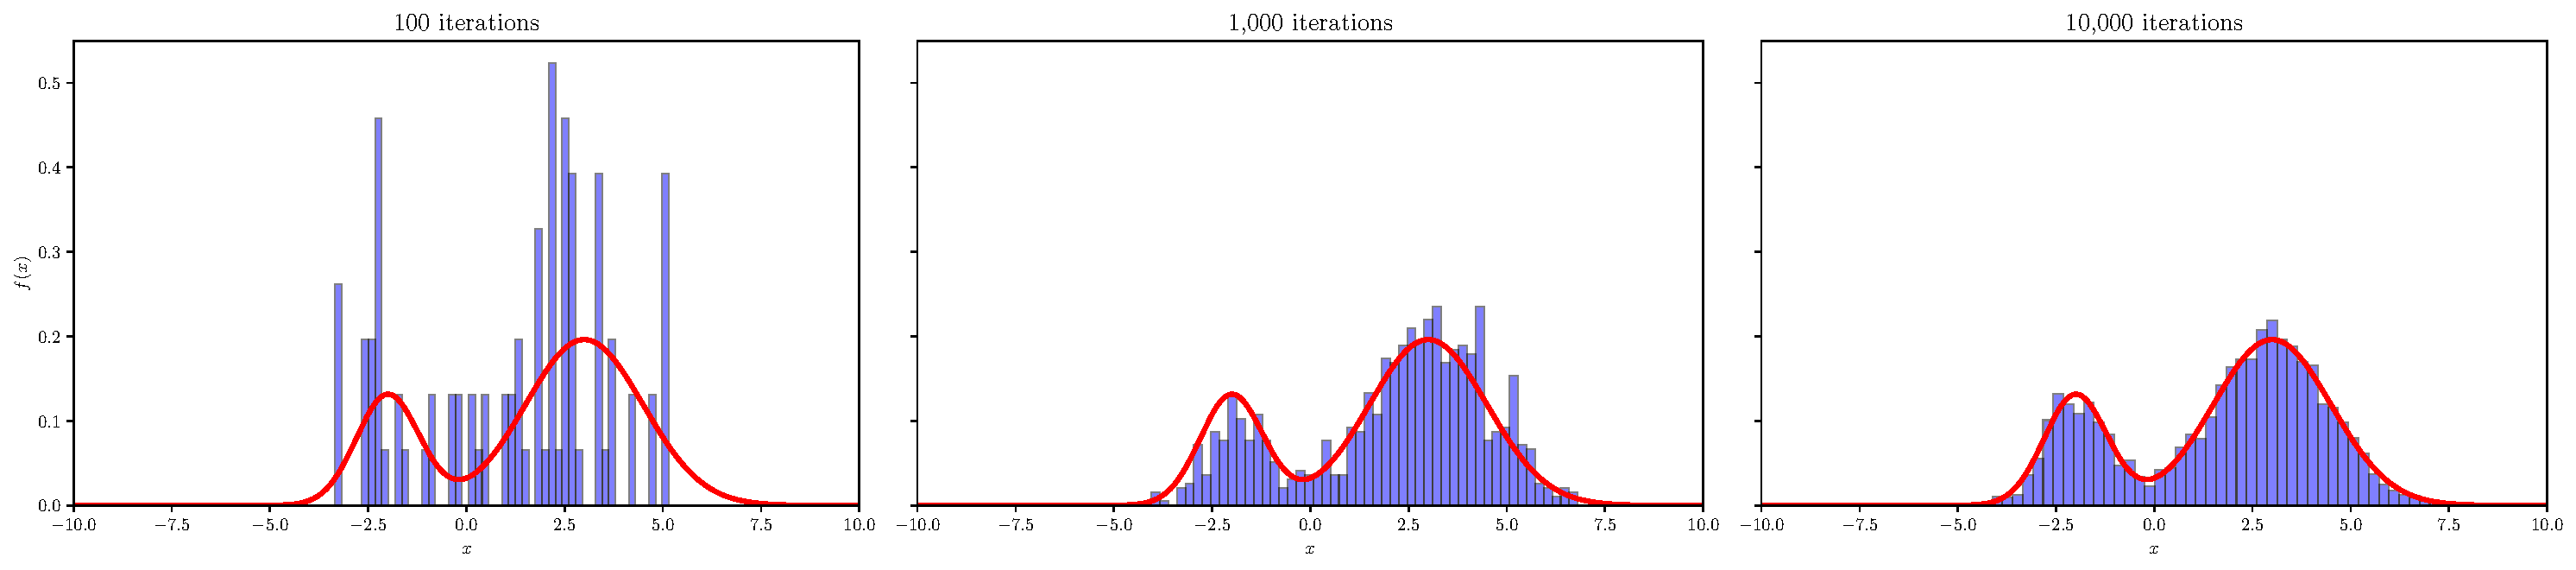
\includegraphics[width=\textwidth]{./figs/monte-carlo/mcmc_convergence.pdf}
    \caption{Convergence of an MCMC sampler. The empirical distribution of samples (histograms) progressively converges to the true target distribution (red line) as the number of iterations increases.}
    \label{fig:mcmc-convergence}
\end{figure}
Figure~\ref{fig:mcmc-convergence} shows this process for a bimodal target distribution (red line). After only 100 iterations, the histogram is a very poor match for the bimodal target distribution. After 1,000, the shape begins to emerge. By 10,000 and 100,000 iterations, the histogram of samples provides an excellent approximation of the true distribution. However, this convergence is not automatic. It is only guaranteed if the Markov chain is \textbf{ergodic}. An ergodic chain has two main properties. First, it is irreducible. This means that every state must be reachable from every other state (perhaps not in one step, but in a finite number of steps). The chain must be able to explore the entire distribution. Second, it is aperiodic. This means that the chain must not get trapped in deterministic cycles (e.g., oscillating between state A and state B forever). Most standard MCMC samplers (like Metropolis-Hastings with a random proposal) are designed to be aperiodic. Irreducibility, however, is a major practical concern.

\begin{warningBox}
    \textbf{Practical Irreducibility and Proposal Choice}

    A chain can be theoretically irreducible but \emph{practically} fail to explore the state space in a reasonable amount of time. This often happens when the target distribution has multiple, well-separated modes (regions of high probability).

    Consider the target distribution $\pi(x) \propto \exp(-(x-10)^2) + 2\exp(-(x+10)^2)$, which has two sharp peaks at $x=-10$ and $x=10$. If we use a small proposal step (e.g., $\Delta x \sim \mathcal{U}(-1, 1)$), the chain will explore one mode (e.g., around $x=10$) very well. However, proposing a jump all the way to $x=-10$ is effectively impossible on practical timescales. The chain gets stuck in one mode and fails to sample the other, even though the chain is technically irreducible. If we use a large proposal step (e.g., $\Delta x \sim \mathcal{U}(-10, 10)$), the chain can propose moves that jump between modes. This allows it to explore the full distribution and sample both modes in their correct proportions (twice as many samples near $x=-10$ as near $x=10$). This is illustrated in Figure~\ref{fig:mcmc-pitfall}. The choice of proposal distribution $M$ is important for ensuring the chain mixes on a practical timescale.

    \begin{figure}[H]
        \centering
        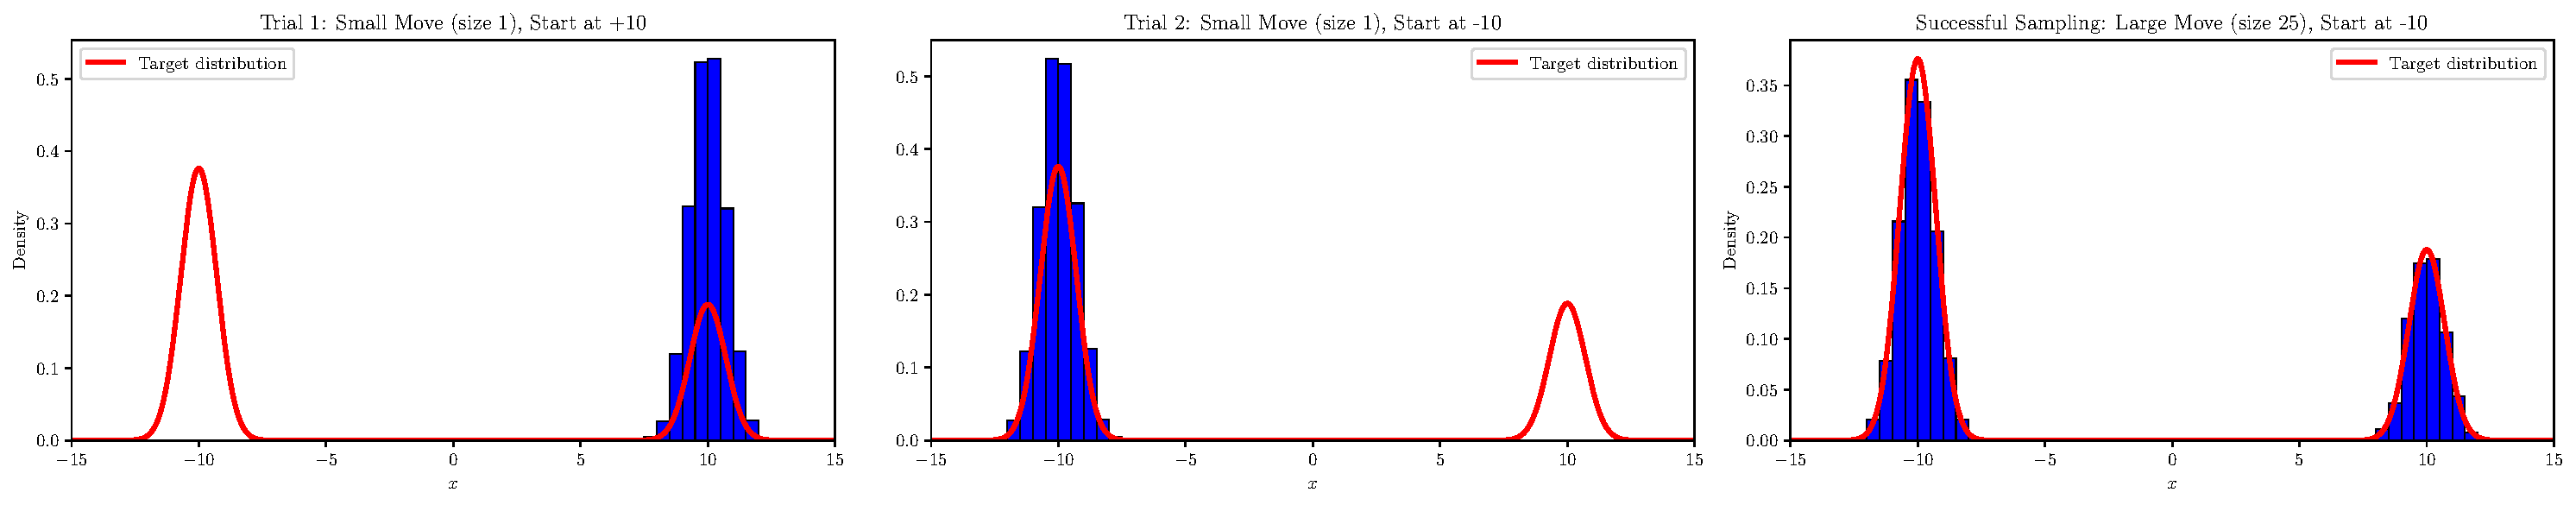
\includegraphics[width=\textwidth]{./figs/monte-carlo/mcmc_pitfall.pdf}
        \caption{The role of the proposal distribution for irreducibility. Left and middle: With a small proposal step (max size 1), the chain gets stuck in whichever mode it starts in (Trial 1 vs. Trial 2). It fails to sample the full distribution. Right: With a large proposal step (large enough to traverse between modes), the chain can jump between the modes at $x=-10$ and $x=10$, correctly sampling the entire target distribution.}
        \label{fig:mcmc-pitfall}
    \end{figure}
\end{warningBox}

\subsection{Practical MCMC}

Running the Metropolis-Hastings algorithm effectively requires handling a few important details carefully. We can use the following techniques to improve the performance of the algorithm.

\paragraph*{Burn-In}
The convergence guarantee of MCMC states that the chain approaches the stationary distribution $\pi(\mathbf{x})$ \emph{in the limit} of infinite steps. However, we must start the chain somewhere. If our initial state $\mathbf{x}_1$ is a bad guess---that is, it lies in a region of very low probability---the first several (or many) steps of the chain will not be representative samples from $\pi(\mathbf{x})$. They instead represent the chain's transient walk towards the high-probability region. To correct for this, we use a process called burn-in. We simply discard some number of initial samples from the MCMC run. For a chain of $M$ total steps, we might discard the first $M_{\text{burn}}$ samples and compute our averages only using the remaining $M - M_{\text{burn}}$ samples, which are more likely to be drawn from the true limiting distribution. Note that when you discard burn-in, you should only use post-burn-in samples for computing expectations. You do not need to further ``thin'' the samples (e.g., keeping only every $k$-th sample) to get correctness; thinning only helps with storage.

\paragraph*{Tempering/Simulated Annealing}
A related challenge, as seen in Figure~\ref{fig:mcmc-pitfall}, is that a chain can get stuck in a local probability mode, failing to explore the full distribution. Tempering is a technique that can help with this. The idea is to first sample from a ``flatter'' version of the target distribution, which is easier to explore, and then gradually ``cool'' the distribution to approach the true one. This is done by introducing an artificial temperature $T_j > 1$ and sampling from $\pi_j(\mathbf{x}) \propto \pi(\mathbf{x})^{1/T_j}$. When $T_j$ is large, $\pi_j(\mathbf{x})$ is much flatter than $\pi(\mathbf{x})$ (Figure~\ref{fig:simulated-annealing-flattening}), allowing the chain to easily jump over probability barriers. The procedure starts with a high $T_1$, runs a chain, then uses its result to initialize a new chain with a smaller $T_2 < T_1$, and so on:
\begin{equation}
    \pi(\mathbf{x})^{1/T_1}, \pi(\mathbf{x})^{1/T_2}, \ldots, \pi(\mathbf{x})^{1/T_M} \quad \text{where} \quad T_1 > T_2 > \cdots > T_M = 1
\end{equation}
The final chain at $T_M=1$ samples from the true target distribution, but it has hopefully been guided to the globally important regions by the previous ``hotter'' chains. 

% MC: hopefully not too confusing, but just thought it might be important to be clear about this (?)
It is worth clarifying terminology. The procedure just described is meant to improve sampling. We gradually cool from a high temperature $T_1$ to
$T_M = 1$ and then keep sampling at $T=1$ to estimate expectations with respect to the true target $\pi(\mathbf{x})$. This idea is closely related to (and historically motivated by) \textbf{simulated annealing}, but the goal of simulated annealing is different. In simulated annealing, we introduce a
temperature $T$ and define a family of tempered distributions $\pi_T(\mathbf{x}) \propto \pi(\mathbf{x})^{1/T}$. We then lower $T$
toward zero, not toward $1$. In the limit $T \to 0$, $\pi_T(\mathbf{x})$ concentrates all of its probability mass on the global maximum of
$\pi(\mathbf{x})$ (or, equivalently, the global minimum of an associated energy or loss function). The Markov chain is run while $T$ is slowly decreased
so that it can escape bad local optima at high temperature but eventually settles into a single best mode at very low temperature. In other words,
simulated annealing is an \emph{optimization} algorithm: it is designed to find the most probable/highest-weight state. By contrast, tempering as used in MCMC for inference does not cool all the way to $T \to 0$. Instead, we stop at $T=1$ and keep sampling so that the chain continues to explore all important regions of $\pi(\mathbf{x})$ in proportion to their probability. In that sense, annealing to $T=0$ is about finding a single answer, while tempering down to $T=1$ is about correctly representing uncertainty across many answers.

\begin{figure}[H]
    \centering
    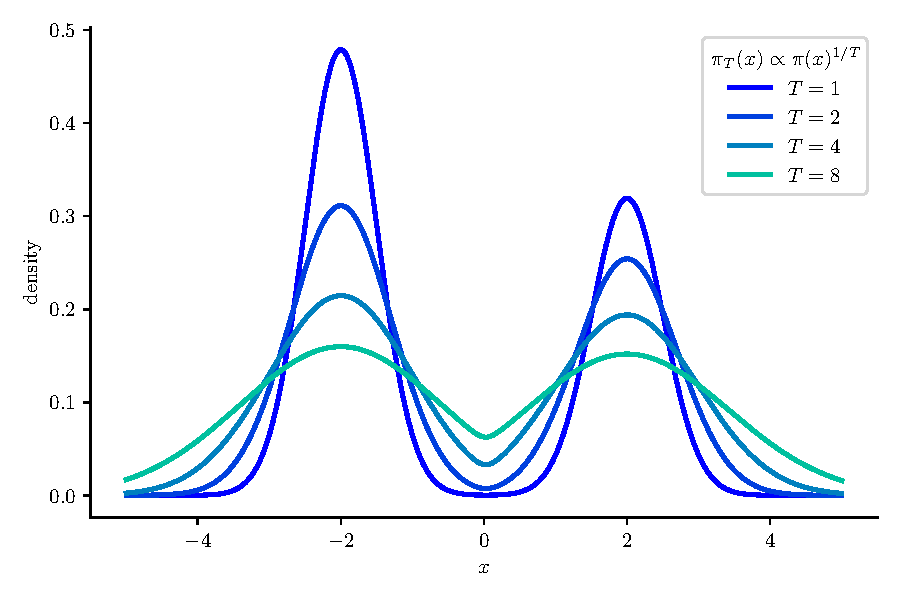
\includegraphics[width=.5\textwidth]{./figs/monte-carlo/simulated_annealing_flattening.pdf}
    \caption{Effect of temperature in tempering. We plot a bimodal target density $\pi(x)$ ($T{=}1$) along with tempered versions $\pi_T(x) \propto \pi(x)^{1/T}$ for hotter temperatures $T>1$. Higher temperatures flatten the distribution, lowering energy barriers between modes and making it easier for an MCMC chain to move between distant regions before cooling back down to $T=1$.}
    \label{fig:simulated-annealing-flattening}
\end{figure}

\begin{warningBox}
    \textbf{Autocorrelation and Effective Sample Size}

    MCMC outputs correlated samples. The estimator $\frac{1}{M}\sum_{i=1}^M f(\mathbf{x}_i)$ is consistent, but its uncertainty depends on the chain's autocorrelation time. Error bars should be based on an \emph{effective} sample size rather than $M$ itself (e.g., via batch means or integrated autocorrelation time). This is not something you'll need to do in 10.34, but it's a good thing to be aware of.
\end{warningBox}

\subsection{Applications}
This brings us back to our original motivation. Why did we start talking about sampling from distributions? To compute expected values. The goal is to compute high-dimensional integrals of the form:
\begin{equation}
    I = \mathbb{E}[f] = \int f(\mathbf{x}) \, \pi(\mathbf{x}) \, d\mathbf{x}
\end{equation}
If we use an MCMC algorithm (like Metropolis-Hastings) to generate a sequence of $M$ samples $\{\mathbf{x}_i\}$ from a chain whose limiting distribution is $\pi(\mathbf{x})$, then by the law of large numbers for Markov chains, the sample mean converges to the true expectation:
\begin{equation}
    I \approx \frac{1}{M} \sum_{i=1}^{M} f(\mathbf{x}_i)
\end{equation}
We replace an intractable high-dimensional integral with a simple average over samples generated from a Markov chain! This lets us solve deterministic integration problems using stochastic sampling methods that greatly mitigate the curse of dimensionality. The error of Monte Carlo integration typically scales like $1/\sqrt{M}$ regardless of dimension, which avoids the exponential growth in grid points required by classical grid-based methods. Figure~\ref{fig:mcmc-2d} illustrates this process in two dimensions. The Markov chain starts at an arbitrary point and performs a random walk that preferentially explores regions of high probability. The trajectory (right panel) may seem random, but over time, the density of the visited points (far right) perfectly reconstructs the target distribution.

\begin{figure}[htbp]
    \centering
    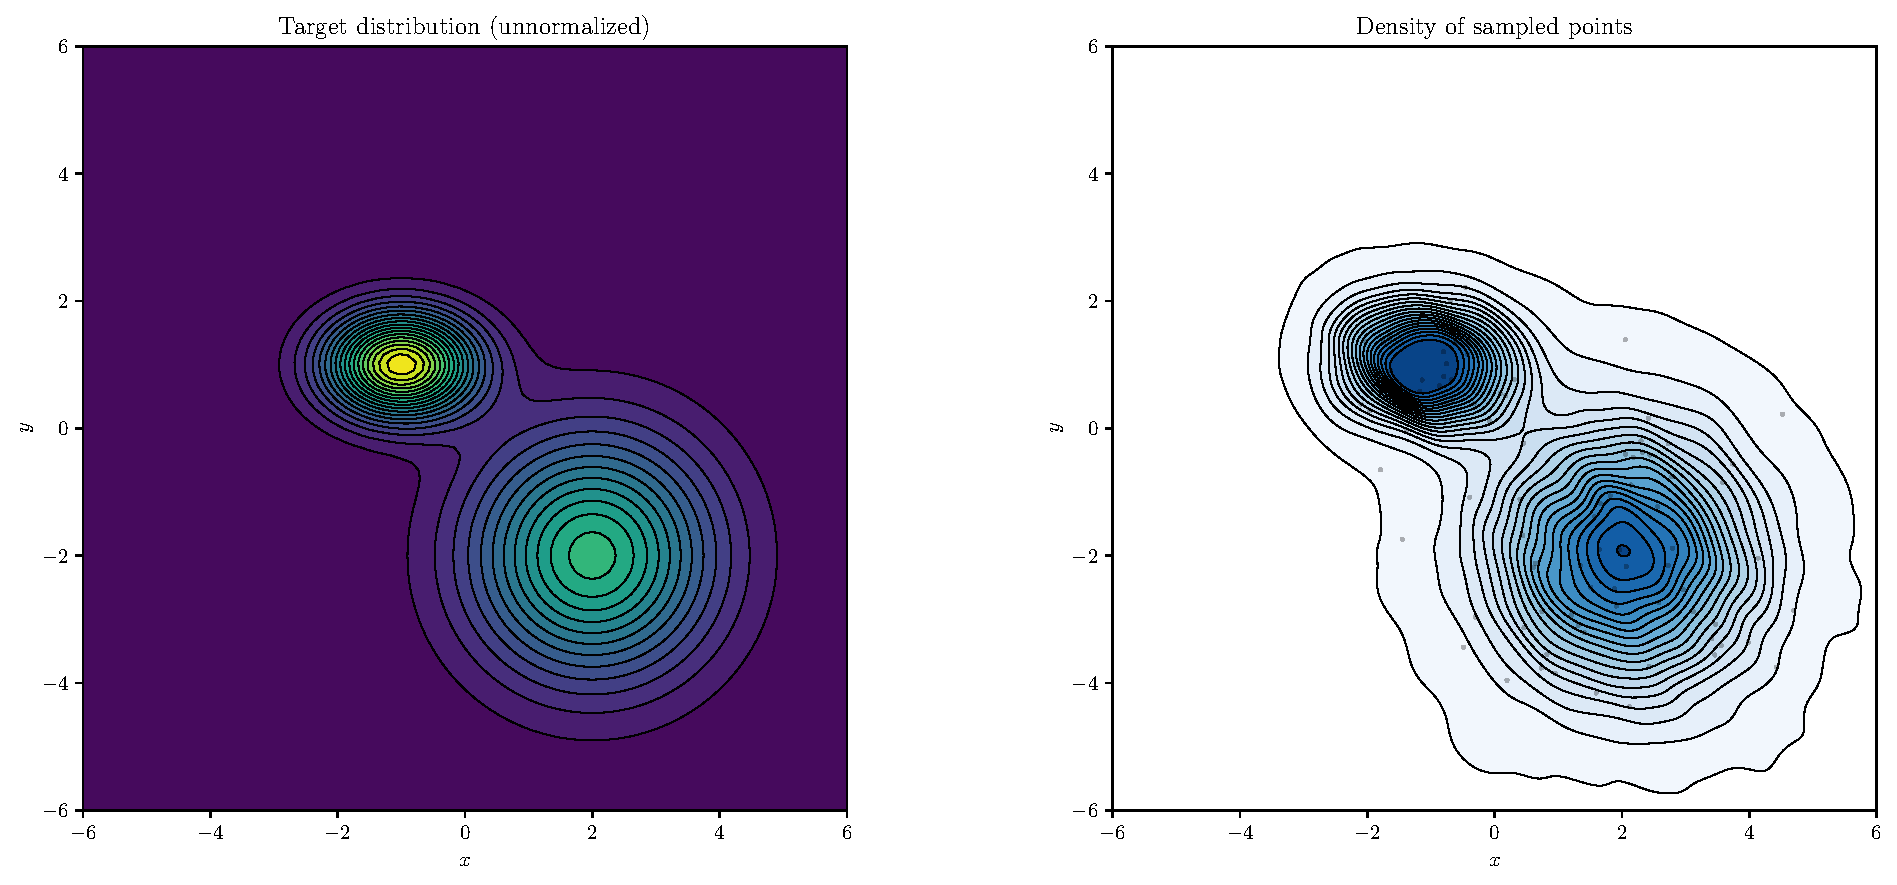
\includegraphics[width=\textwidth]{./figs/monte-carlo/mcmc_2d.pdf}
    \caption{MCMC in two dimensions. The algorithm explores the state space, and the density of the samples converges to the target distribution.}
    \label{fig:mcmc-2d}
\end{figure}

The single most important feature of MCMC, which we have already used and stated a couple times before, is that the acceptance probability depends only on the ratio of probabilities. This means we never need to know the normalization constant $Z$. We can work directly with any unnormalized function $w(\mathbf{x})$ that is proportional to our target distribution, $\pi(\mathbf{x}) \propto w(\mathbf{x})$. Our goal is to compute expectations $\langle f \rangle = \int f(\mathbf{x}) \pi(\mathbf{x}) d\mathbf{x}$. Using the unnormalized weight $w(\mathbf{x})$, this is
\begin{equation}
    \langle f \rangle = \frac{\int f(\mathbf{x}) w(\mathbf{x}) d\mathbf{x}}{\int w(\mathbf{x}) d\mathbf{x}}
\end{equation}
But the MCMC samples $\{\mathbf{x}_i\}$ are drawn with a probability proportional to $w(\mathbf{x})$ precisely to handle this. The simple average of $f$ over the MCMC samples correctly estimates this value:
\begin{equation}
    \langle f \rangle \approx \frac{1}{M} \sum_{i=1}^{M} f(\mathbf{x}_i)
\end{equation}
We'll now look at applying MCMC to statistical mechanics and Bayesian parameter estimation, which are two of MCMC's most powerful applications.

\paragraph*{Statistical Mechanics}
In statistical mechanics, the probability of a system being in a state $\mathbf{q}$ (with energy $U(\mathbf{q})$) is given by the Boltzmann distribution:
\begin{equation}
    \pi(\mathbf{q}) = \frac{1}{Z} \exp\left(-\frac{U(\mathbf{q})}{k_B T}\right)
\end{equation}
where $k_B$ is Boltzmann's constant and $T$ is the temperature. Here, $w(\mathbf{q}) = \exp(-U(\mathbf{q})/k_B T)$ is the unnormalized weight. We can compute the expectation of any quantity (like energy, $\langle U \rangle = \int U(\mathbf{q})\,\pi(\mathbf{q})\,d\mathbf{q}$) by sampling from $\pi(\mathbf{q})$ using MCMC.
For a symmetric proposal $\mathbf{q}_i \to \mathbf{q}^*$, the Metropolis acceptance probability simplifies to
\begin{align}
    A(\mathbf{q}^*, \mathbf{q}_i) &= \min \left\{ 1, \frac{\pi(\mathbf{q}^*)}{\pi(\mathbf{q}_i)} \right\}
    = \min \left\{ 1, \frac{\exp(-U(\mathbf{q}^*)/k_B T)}{\exp(-U(\mathbf{q}_i)/k_B T)} \right\} \\
    &= \min \left\{ 1, \exp\left(-\frac{U(\mathbf{q}^*) - U(\mathbf{q}_i)}{k_B T}\right) \right\} = \min \left\{ 1, \exp\left(-\frac{\Delta U}{k_B T}\right) \right\}
\end{align}
The decision to accept a move depends \emph{only on the change in energy} $\Delta U = U(\mathbf{q}^*) - U(\mathbf{q}_i)$. This makes a lot of physical sense! If the energy goes down (i.e., $\Delta U < 0 \implies \exp(-\Delta U/k_B T) > 1$), we always accept the move. If the energy goes up (i.e., $\Delta U > 0 \implies \exp(-\Delta U/k_B T) < 1$), we accept the move with some probability that depends on the difference in energy and the temperature.

\paragraph*{Bayesian Parameter Estimation}
In parameter estimation, our target distribution is the posterior:
\begin{equation}
    p(\boldsymbol{\theta}|\mathcal{D}) = \frac{1}{Z} p(\mathcal{D}|\boldsymbol{\theta}) p(\boldsymbol{\theta})
\end{equation}
Assuming a Gaussian likelihood, $p(\mathcal{D}|\boldsymbol{\theta}) \propto \exp(-\chi^2(\boldsymbol{\theta})/2)$. The unnormalized posterior is $w(\boldsymbol{\theta}) = \exp(-\chi^2(\boldsymbol{\theta})/2) p(\boldsymbol{\theta})$.
The Metropolis acceptance probability for a symmetric proposal $\boldsymbol{\theta}_i \to \boldsymbol{\theta}^*$ is:
\begin{align}
    A(\boldsymbol{\theta}^*, \boldsymbol{\theta}_i) &= \min \left\{ 1, \frac{p(\boldsymbol{\theta}^*|\mathcal{D})}{p(\boldsymbol{\theta}_i|\mathcal{D})} \right\}
    = \min \left\{ 1, \frac{\exp(-\chi^2(\boldsymbol{\theta}^*)/2) p(\boldsymbol{\theta}^*)}{\exp(-\chi^2(\boldsymbol{\theta}_i)/2) p(\boldsymbol{\theta}_i)} \right\} \\
    &= \min \left\{ 1, \frac{p(\boldsymbol{\theta}^*)}{p(\boldsymbol{\theta}_i)} \exp\left(-\frac{\chi^2(\boldsymbol{\theta}^*) - \chi^2(\boldsymbol{\theta}_i)}{2}\right) \right\}
\end{align}
The acceptance probability depends only on the change in the weighted sum of squared errors and the ratio of the prior. If the prior is uniform, $p(\boldsymbol{\theta}^*) = p(\boldsymbol{\theta}_i)$, it depends only on the change in $\chi^2$. Once we have run the chain and collected samples $\{\boldsymbol{\theta}_i\}$, we can do much more than just find the mean. We can ask/answer any question about the posterior distribution:
\begin{itemize}
    \item Marginalization: To find $p(\theta_1|\mathcal{D})$, we simply make a histogram of the $\theta_1$ components of all our samples.
    \item Credible intervals: What is the probability that a parameter $\theta_j$ is in a certain region $\Omega$? We just count the samples: $P(\theta_j \in \Omega) \approx \frac{1}{M} \sum_{i=1}^M \mathbb{I}(\theta_{i,j} \in \Omega)$, where $\mathbb{I}$ is the indicator function.
    \item Prediction: What value $y$ might we measure for a new input $x$? We can generate a predictive distribution by taking each sample $\boldsymbol{\theta}_i$ and drawing a corresponding $y$ from the model: $y_i = g(x; \boldsymbol{\theta}_i) + \epsilon_i$, where $\epsilon_i$ is drawn from the measurement noise. The histogram of $\{y_i\}$ shows our full prediction.
\end{itemize}

%%% Local Variables:
%%% mode: LaTeX
%%% TeX-master: "../main"
%%% End: